\documentclass[11pt]{article}

\usepackage[margin=1in]{geometry}
\usepackage{graphicx}
\usepackage{array}
\usepackage{tabularx}
\usepackage{longtable}
\usepackage{booktabs}
\usepackage{enumitem}
\usepackage{fancyhdr}
\usepackage[dvipsnames]{xcolor}
\usepackage{hyperref}
\usepackage{float}
\usepackage{caption}
\usepackage{subcaption}
\usepackage{listings}
\usepackage{tikz}
\usepackage[most]{tcolorbox}
\usepackage{siunitx}
\usepackage[all]{nowidow}
\usepackage{needspace}
\usepackage{etoolbox}
\usetikzlibrary{arrows.meta,positioning,calc,fit,shapes.misc}

\hypersetup{
  colorlinks=true,
  linkcolor=MidnightBlue,
  urlcolor=MidnightBlue,
  pdftitle={EE301 Microcontroller Laboratory},
  pdfauthor={Arthur Chu}
}

\pagestyle{fancy}
\setlength{\headheight}{14pt}
\fancyhf{}
\lhead{EE301 -- Fundamentals of Electrical Engineering}
\rhead{AY26-2}
\lfoot{Microcontroller Laboratory}
\rfoot{\thepage}
\renewcommand{\headrulewidth}{0.4pt}
\renewcommand{\footrulewidth}{0.4pt}

\captionsetup{font=small, labelfont=bf}
\setlength{\parindent}{0pt}
\setlength{\parskip}{0.4em}
\setcounter{secnumdepth}{2}

\definecolor{Accent}{HTML}{153E5C}
\definecolor{SoftAccent}{HTML}{EAF1F6}
\definecolor{WarnBg}{HTML}{FFF4E5}
\definecolor{WarnFrame}{HTML}{C77D1A}
\definecolor{NoteBg}{HTML}{EEF7EE}
\definecolor{NoteFrame}{HTML}{4B8A5B}
\definecolor{CodeBg}{HTML}{F6F8FA}
\definecolor{LightGray}{HTML}{707070}

\newtcolorbox{warningbox}{
  colback=WarnBg,
  colframe=WarnFrame,
  boxrule=0.8pt,
  arc=2pt,
  left=8pt,right=8pt,top=6pt,bottom=6pt
}

\newtcolorbox{notebox}{
  colback=NoteBg,
  colframe=NoteFrame,
  boxrule=0.8pt,
  arc=2pt,
  left=8pt,right=8pt,top=6pt,bottom=6pt
}

\newtcolorbox{calloutbox}[1]{
  colback=SoftAccent,
  colframe=Accent,
  title=#1,
  fonttitle=\bfseries,
  boxrule=0.8pt,
  arc=2pt,
  left=8pt,right=8pt,top=6pt,bottom=6pt
}

\lstdefinestyle{pycode}{
  language=Python,
  basicstyle=\ttfamily\small,
  keywordstyle=\color{MidnightBlue}\bfseries,
  commentstyle=\color{OliveGreen},
  stringstyle=\color{BrickRed},
  showstringspaces=false,
  frame=single,
  framerule=0.5pt,
  backgroundcolor=\color{CodeBg},
  columns=fullflexible,
  keepspaces=true,
  breaklines=true,
  tabsize=4,
  xleftmargin=0.5em,
  xrightmargin=0.5em,
  aboveskip=0.6em,
  belowskip=0.6em
}
\lstset{style=pycode}

\preto\section{\Needspace{6\baselineskip}}
\preto\subsection{\Needspace{5\baselineskip}}
\preto\subsubsection{\Needspace{4\baselineskip}}
\BeforeBeginEnvironment{lstlisting}{\Needspace{12\baselineskip}}
\BeforeBeginEnvironment{verbatim}{\Needspace{14\baselineskip}}

\newcommand{\kit}[1]{\texttt{#1}}

\begin{document}

\begin{center}
{\Large \textbf{EE301 Microcontroller Laboratory}}\\[0.25em]
{\large \textbf{Board Setup, CircuitPython Basics, and microSD Logging}}
\end{center}

This lab introduces board assembly, Bluefruit reflash, Visual Studio Code setup, basic CircuitPython interaction, NeoPixel control, and temperature logging to a microSD card. The skills introduced in this lab will form the foundation for your final project.

\begin{calloutbox}{Learning Objectives}
By the end of this lab, you should be able to:
\begin{enumerate}
    \item safely assemble the PCB and mount the Circuit Playground Bluefruit,
    \item place the Bluefruit in bootloader mode and run the provided reflash script to restore it to the course baseline image,
    \item use Visual Studio Code to edit \kit{code.py} and view serial output,
    \item read onboard sensor data and control onboard outputs, and
    \item write time-varying sensor data to a text file on a microSD card.
\end{enumerate}
\end{calloutbox}

\begin{figure}[H]
\centering
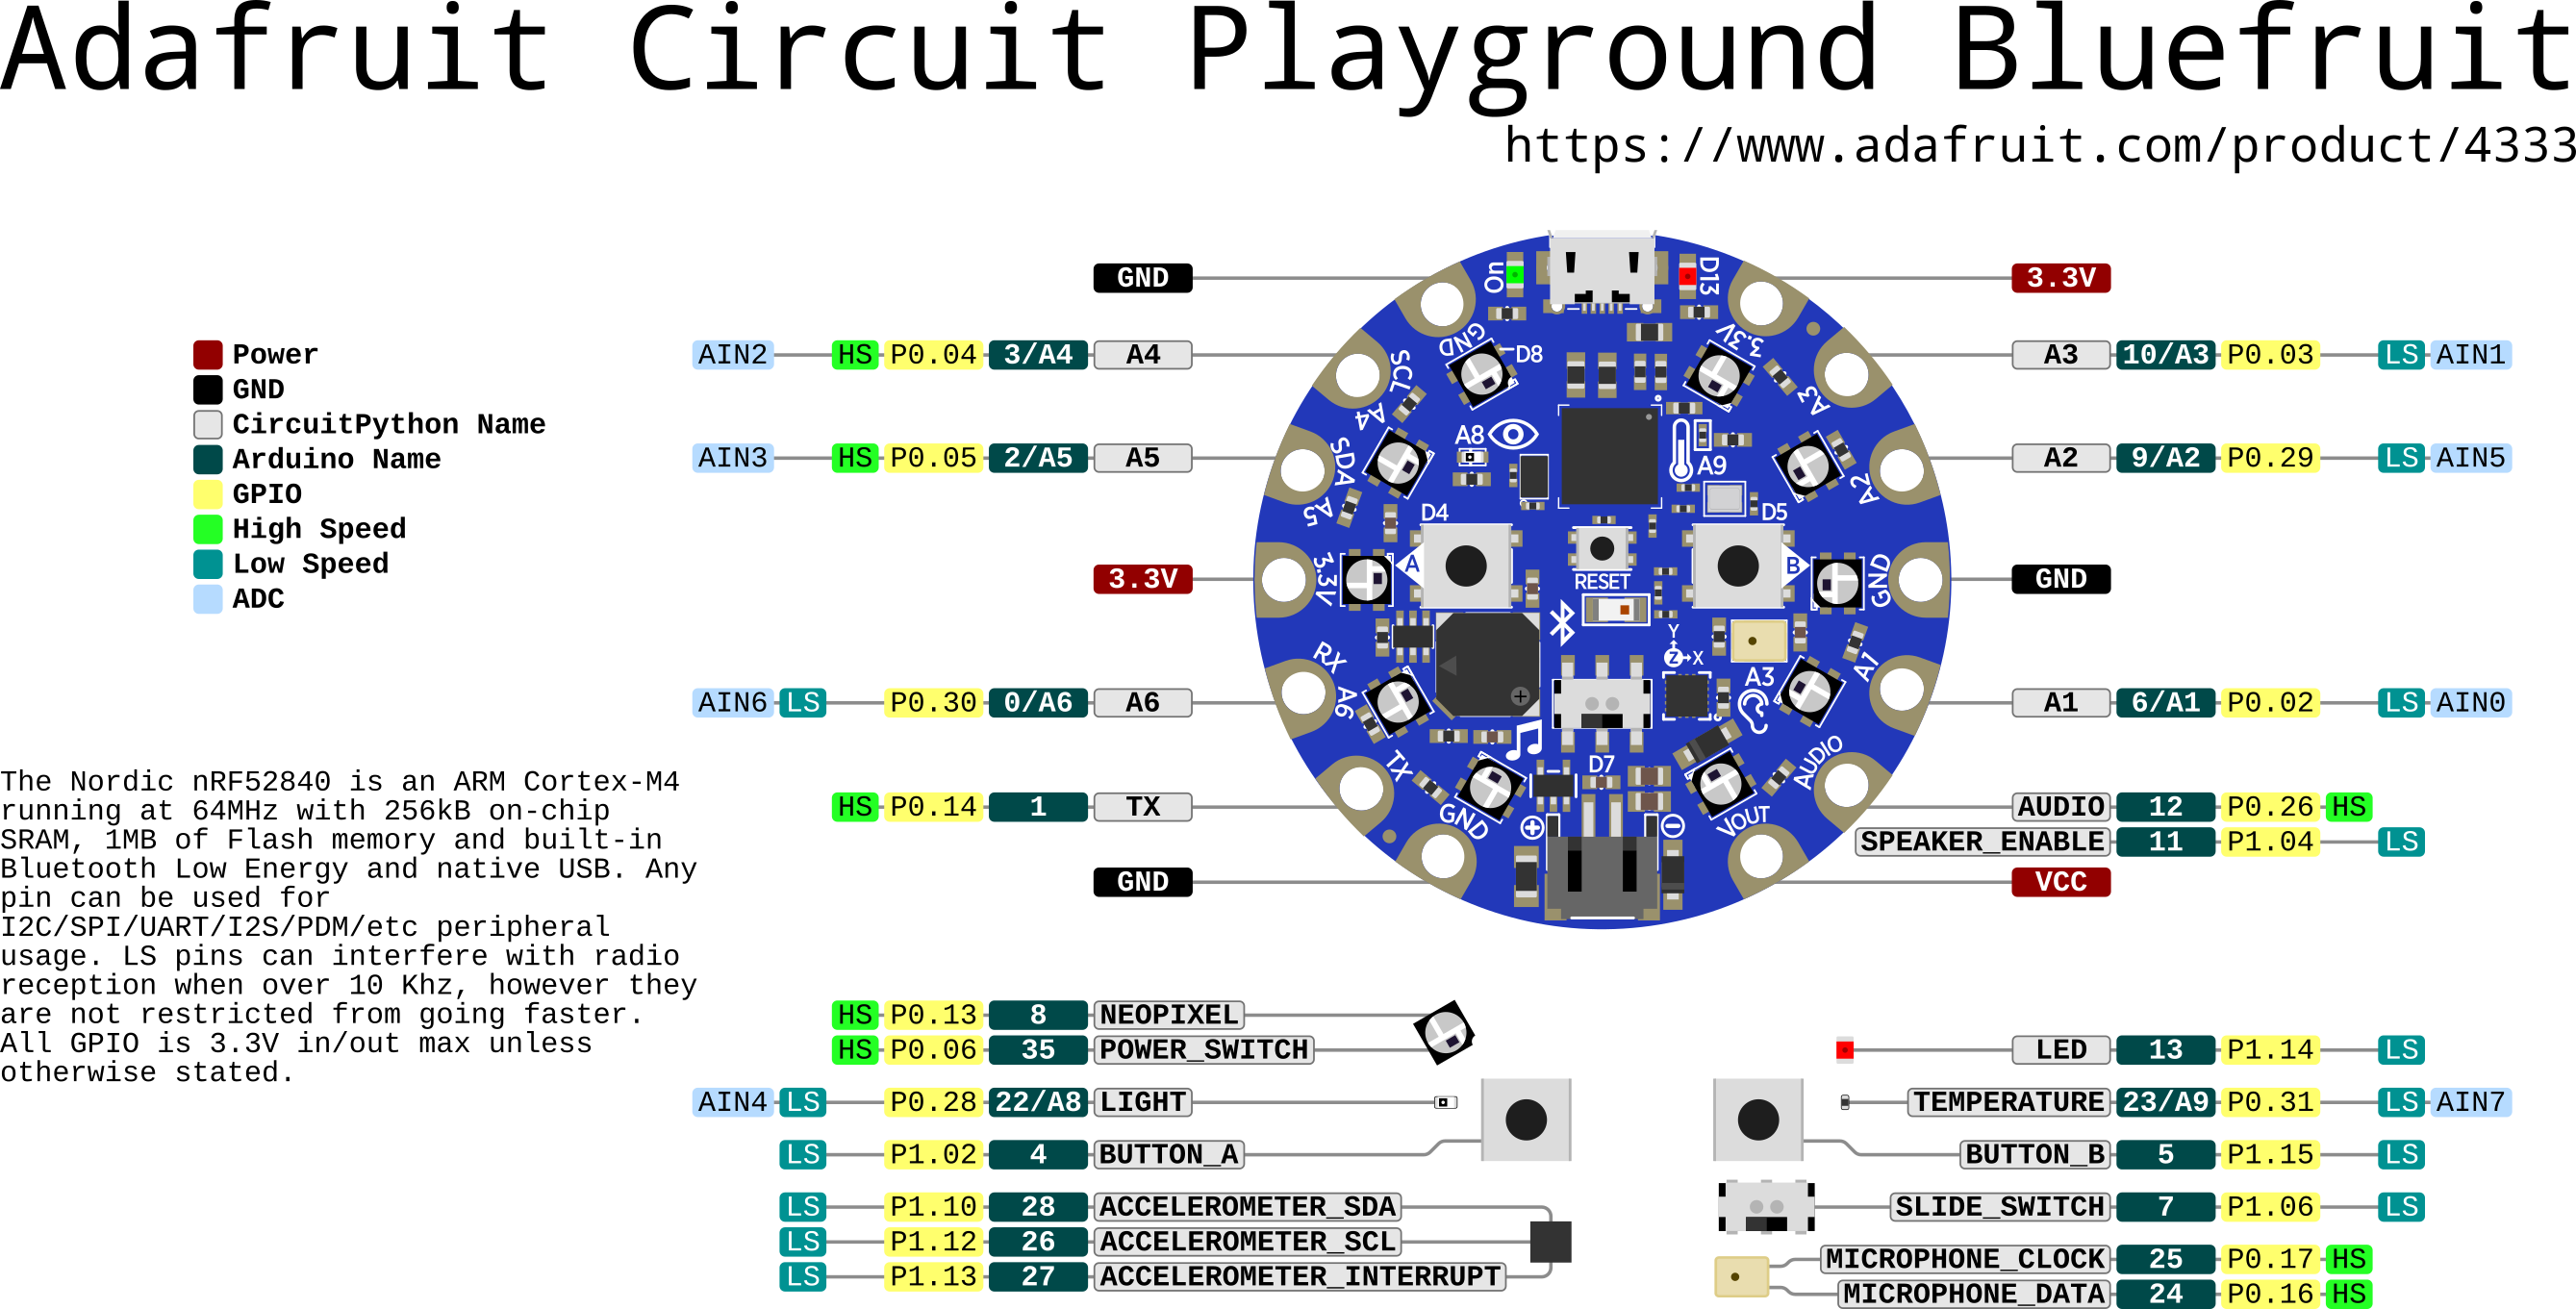
\includegraphics[width=0.9\linewidth]{assets/bluefruit_pinout.png}
\caption{Circuit Playground Bluefruit pinout reference. Keep this page handy when connecting external devices.}
\end{figure}

\section*{Required equipment}
\begin{itemize}
    \item Personal laptop
    \item CY105/EE301 carrier PCB
    \item Adafruit Circuit Playground Bluefruit
    \item USB-A to micro-USB cable
    \item 12-pin male header for the carrier PCB
    \item Small screwdriver and pliers
    \item 12 sets of nuts and bolts
    \item Soldering iron set to approximately \SI{750}{\degree F}
    \item Solder and a ventilating fan
    \item Eye protection
    \item MicroSD breakout board, 4 jumper wires, and microSD card
\end{itemize}

\begin{warningbox}
\textbf{Don't become a statistic!} Wear eye protection. Use the fan. Solder may contain lead. Either feed the solder with pliers or wash your hands thoroughly after handling it and before eating. Do not leave the iron unattended on the bench. Unplug and stow the iron after use.
\end{warningbox}

\section{Setting up hardware}

\subsection{Install Visual Studio Code}
Download and begin installing Visual Studio Code on your laptop. The installer can be found at \url{https://code.visualstudio.com/download}. Let the installer run in the background while you complete the hardware assembly steps below.

%\begin{notebox}
%A long-running installer should not hold up the rest of the lab. 
%We will revisit Visual Studio Code after the Bluefruit hardware has been assembled.
%\end{notebox}

\subsection{Solder the 12-pin header onto the carrier PCB}
Insert the 12-pin male header into the carrier PCB from the \textbf{front side} so that the pins protrude from the side marked \textbf{Beat Navy!}. The soldering itself must be performed on the \textbf{Beat Navy!} side.

\begin{figure}
\centering
\begin{subfigure}[t]{0.48\linewidth}
    \centering
    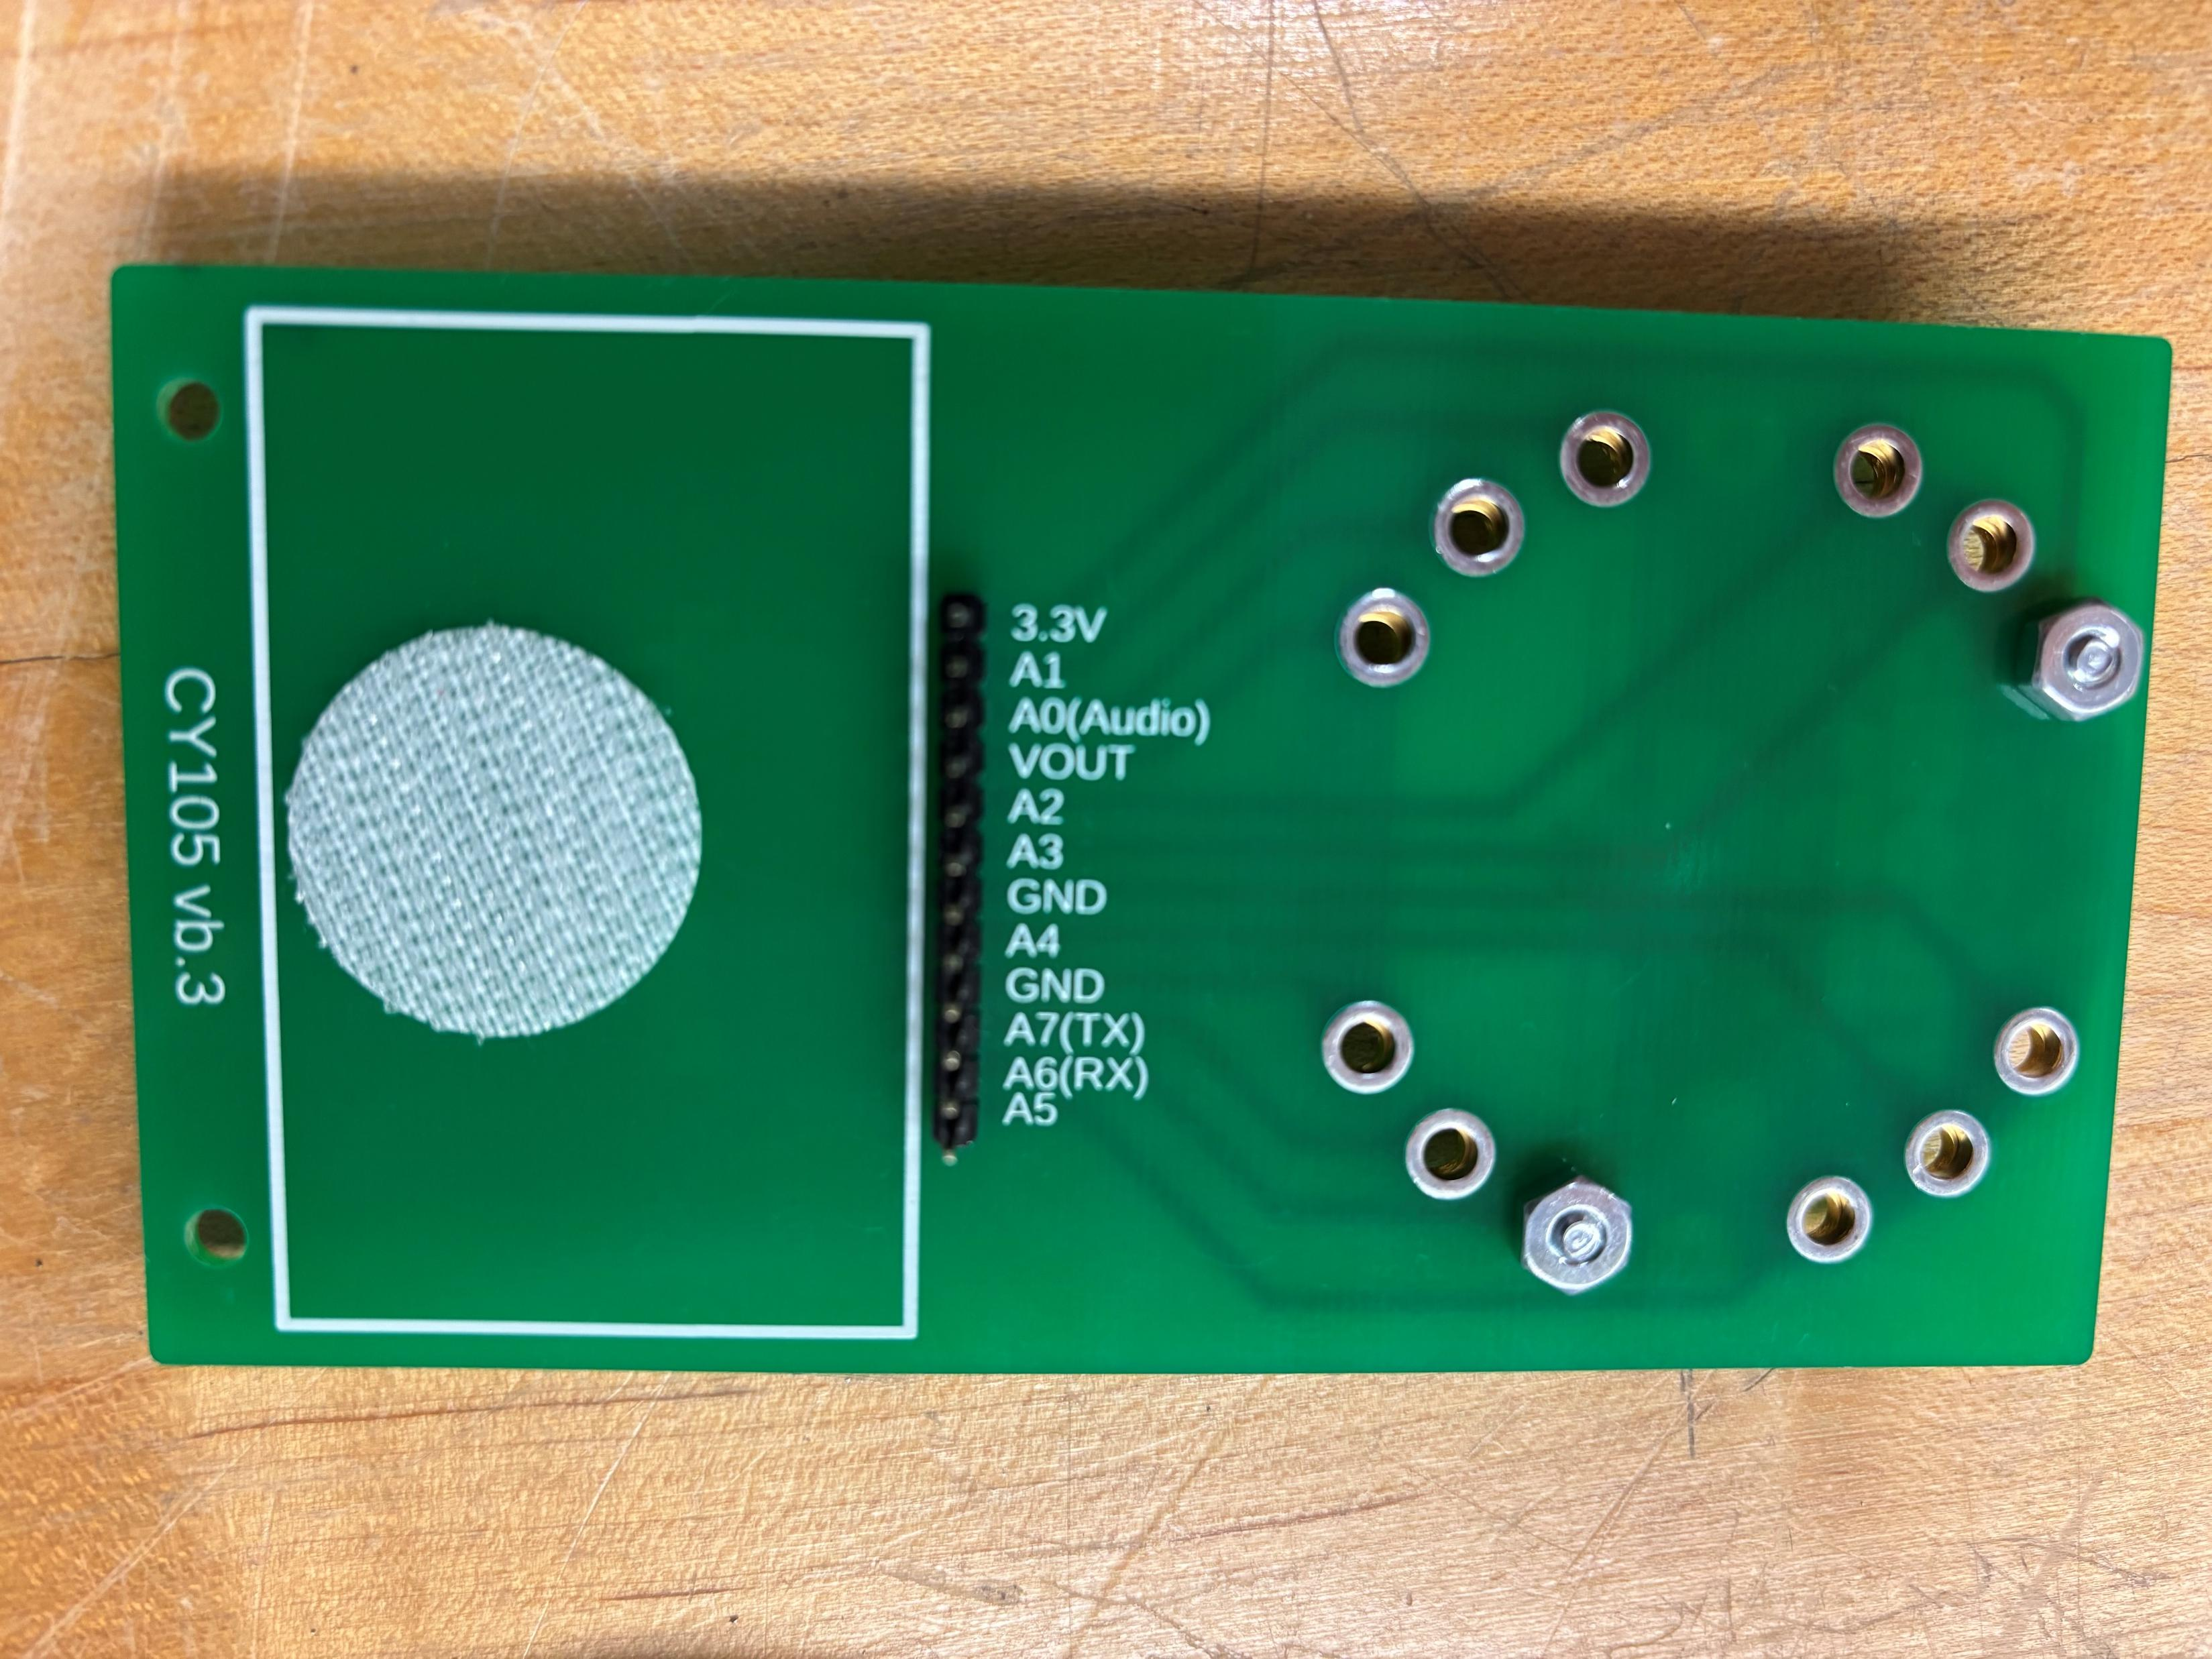
\includegraphics[width=\linewidth]{assets/reverse_side.jpg}
    \caption{Front side: insert the header from this side.}
\end{subfigure}
\hfill
\begin{subfigure}[t]{0.48\linewidth}
    \centering
    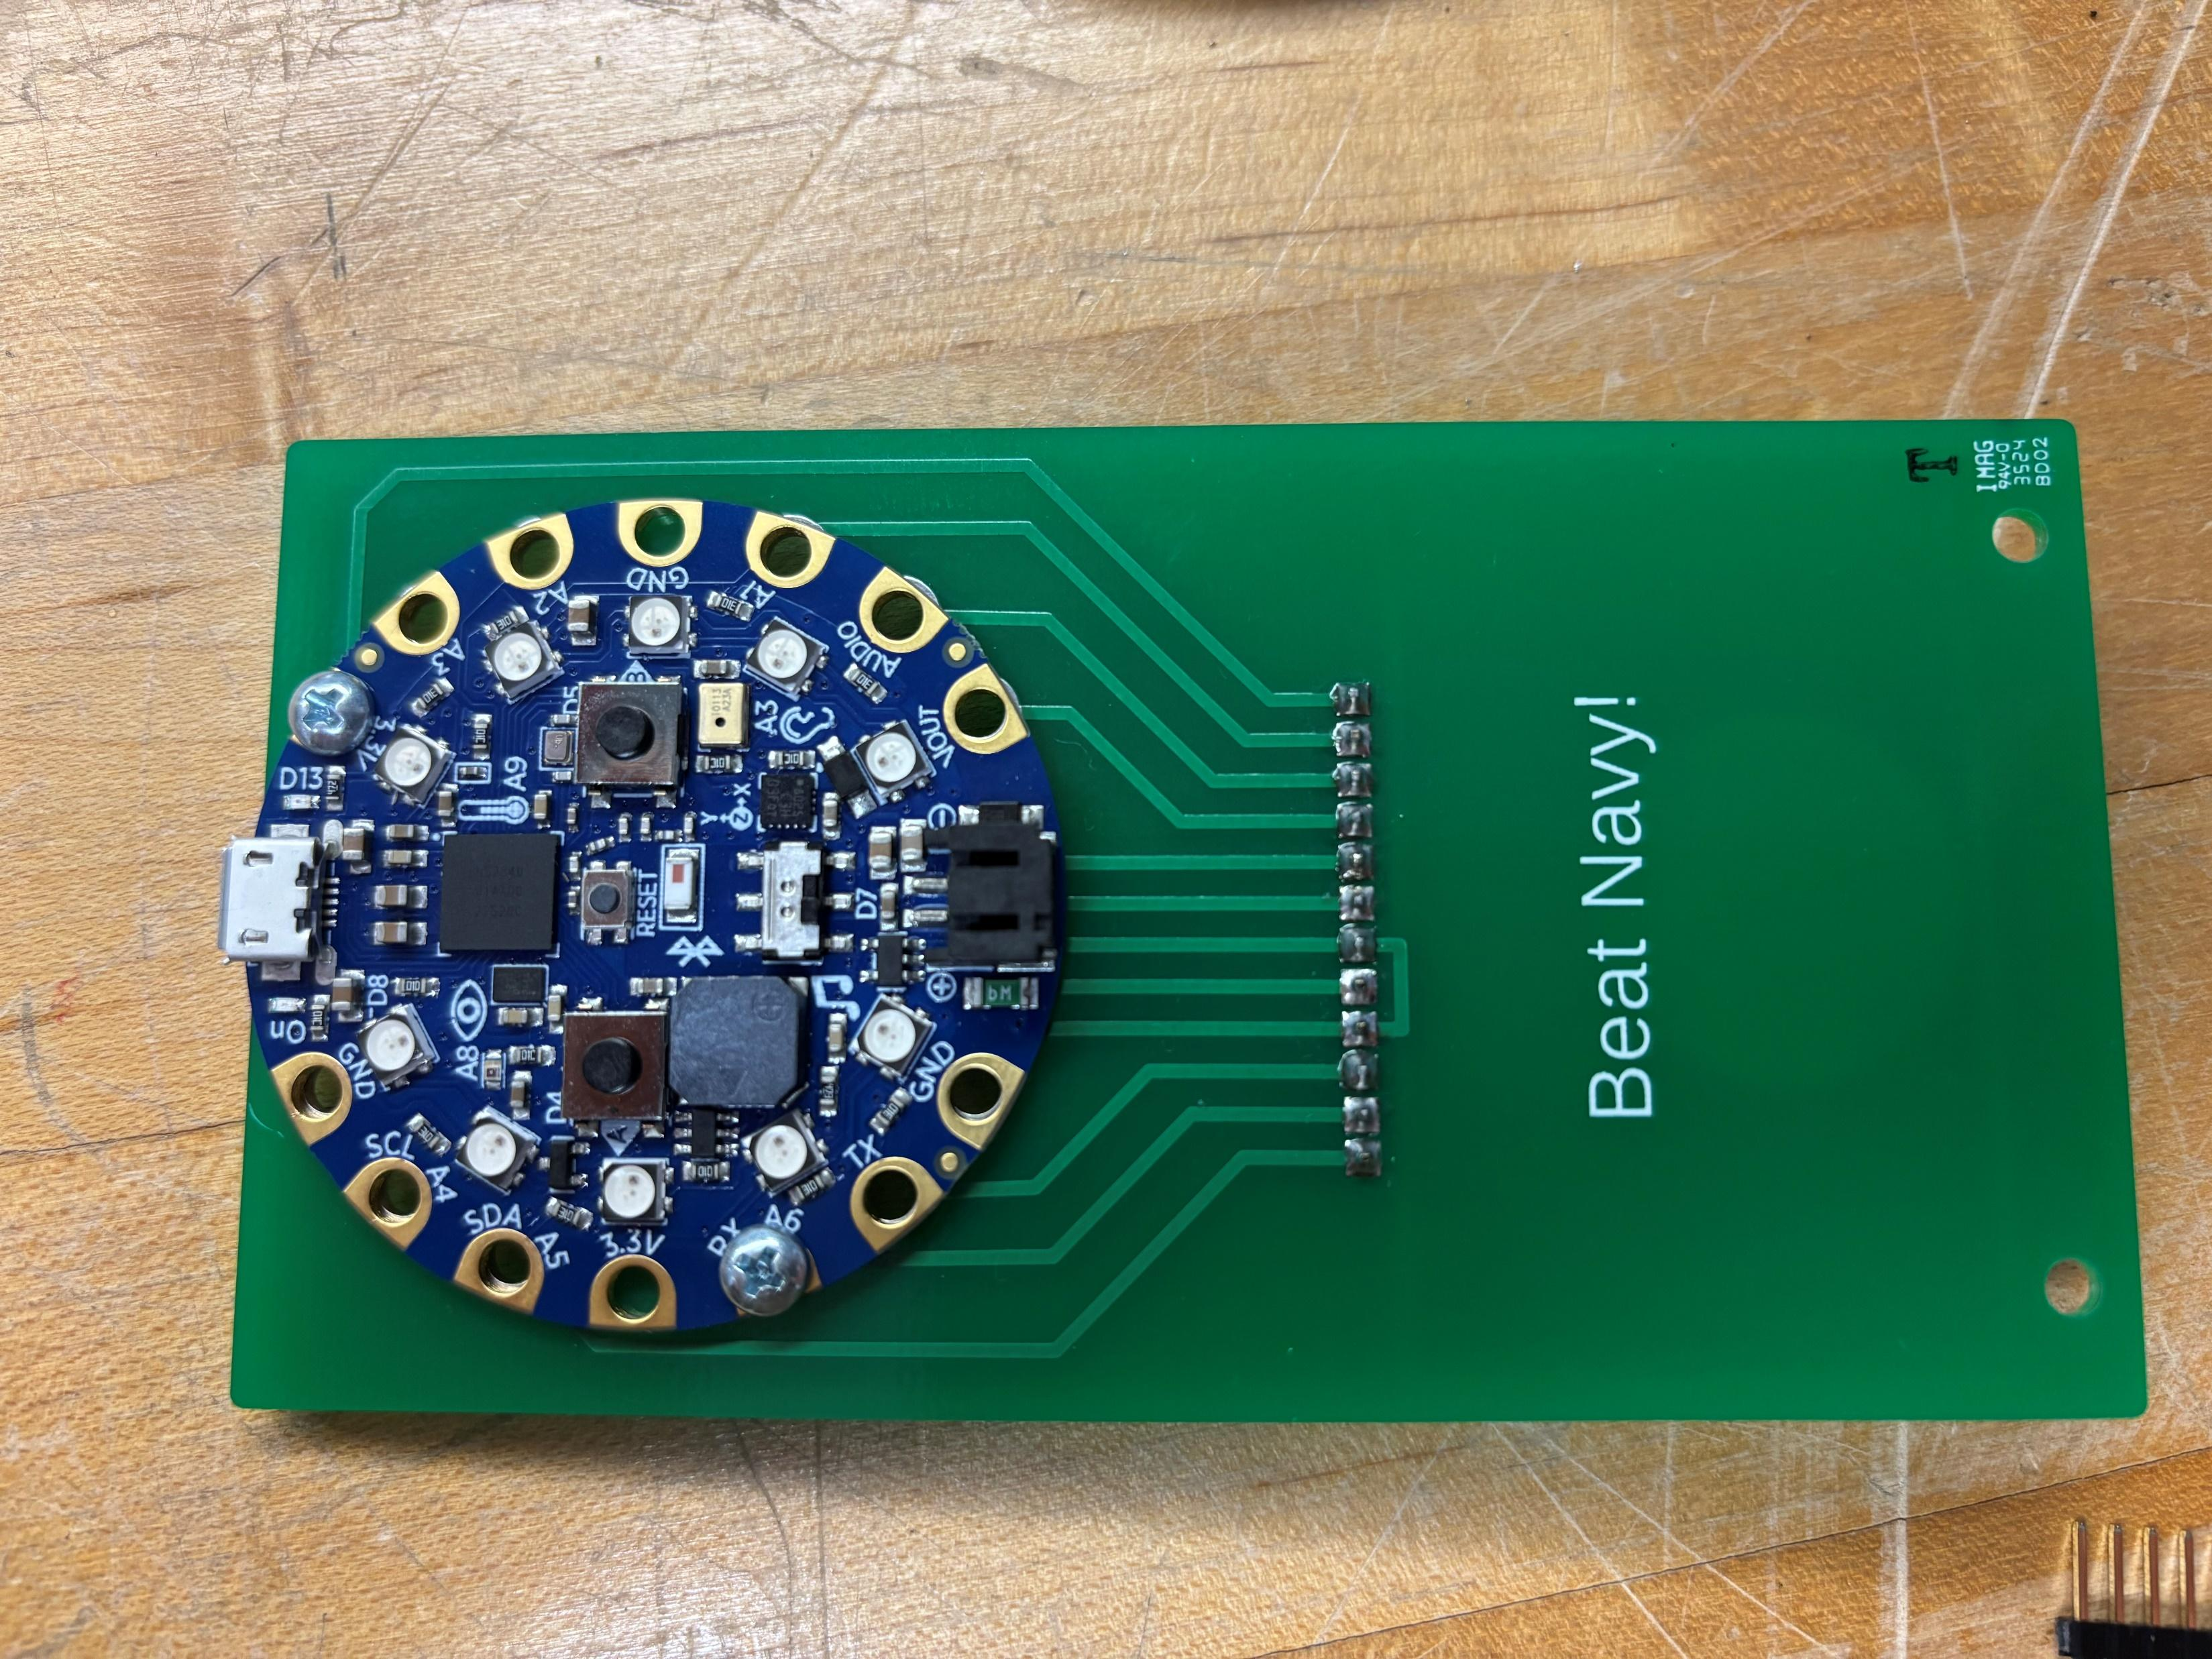
\includegraphics[width=\linewidth]{assets/beat_navy_side.jpg}
    \caption{Beat Navy! side: the pins protrude here, solder here, and mount the Bluefruit here.}
\end{subfigure}
\caption{Carrier PCB orientation during assembly.}\label{fig:pcb}
\end{figure}

\textbf{Soldering procedure}
\begin{enumerate}
    \item Insert the header through the small row of holes from the front side, as shown in Figure~\ref{fig:pcb}.
    \item Solder the first pin.
    \item Recheck alignment before soldering the remaining pins.
    \item Inspect the completed row before moving on.
\end{enumerate}

\textbf{Helpful tips.}
\begin{itemize}
    \item Heat both the pad and the pin, then feed solder into the joint.
    \item Use only enough solder to form a small fillet. More solder is not a better joint.
    \item If the header will not stay square, temporarily hold it with a breadboard, tape, or helping hands.
    \item If two neighboring pins are bridged, reheat and wick away the excess solder before continuing.
\end{itemize}

\begin{figure}
\centering
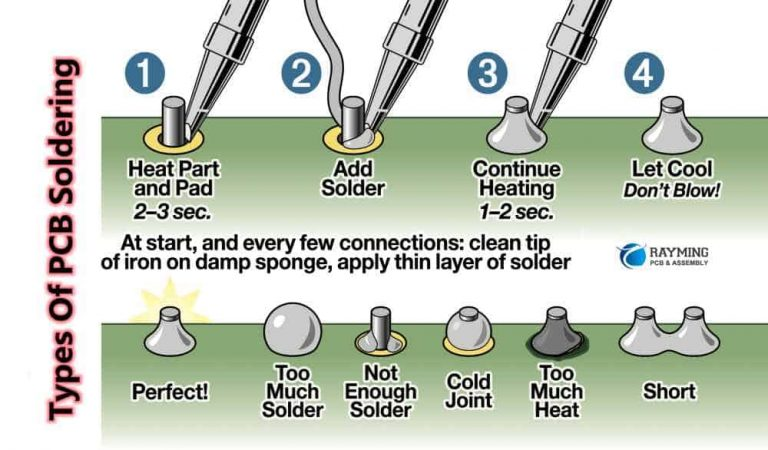
\includegraphics[width=.92\linewidth]{assets/soldering_procedure.png}
\caption{Soldering procedure. Note how the soldering iron is in contact with both the pin and pad in the first step.}
\label{fig:soldering_procedure}
\end{figure}

\begin{figure}
\centering
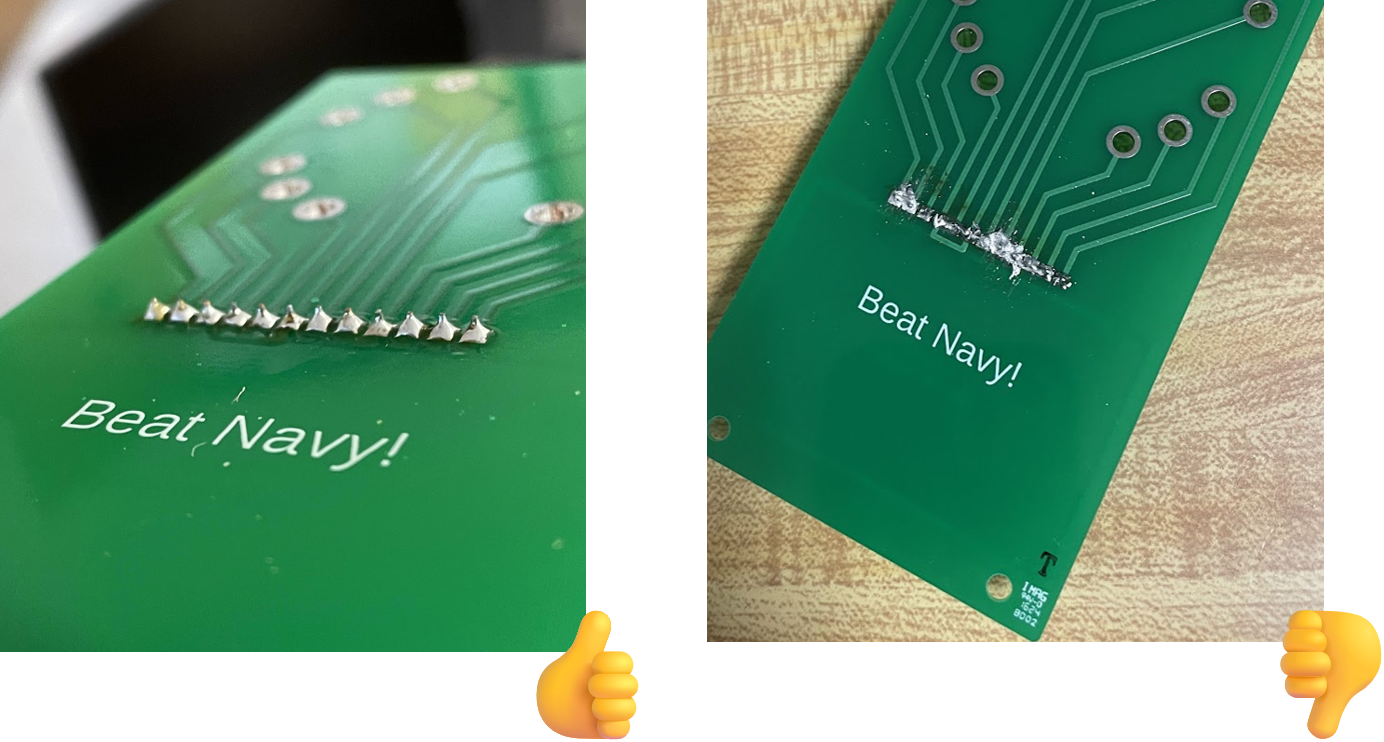
\includegraphics[width=.75\linewidth]{assets/soldering_examples.png}
\caption{Examples of good and bad soldering joints. Note the bridging on the right from using an excessive amount of solder.}
\label{fig:soldering_example}
\end{figure}

\subsection{Mount the Bluefruit onto the carrier PCB}
Once the header soldering is complete and satisfactory, mount the Adafruit Circuit Playground Bluefruit to the carrier PCB using the provided nuts and bolts. The Bluefruit belongs on the same side as the \textbf{Beat Navy!} text and the header pins.

\begin{itemize}
    \item Use a screwdriver on the screw head and pliers on the nut.
    \item Tighten until the board is snug and there is no play.
    \item Do not overtighten. The board should be secure, not crushed.
    \item Confirm that the micro USB connector is pointed \textbf{up} on the carrier board, sitting on its top edge.
\end{itemize}

\begin{warningbox}
\textbf{Did you get it right?} Before tightening fully, verify that the Bluefruit is on the correct side of the carrier PCB. If it is mounted on the wrong side, the labeled header row will not correspond to the board pads as intended.
\end{warningbox}

\subsection{Power the Bluefruit from your laptop}
Use the USB-A to micro-USB cable to connect the Bluefruit to your laptop. The board should power up immediately.

\subsection{Enter bootloader mode}
Double-tap the small reset button in the center of the Bluefruit to enter bootloader mode. In this mode, the outer NeoPixels should turn red briefly before turning solid green, and your computer should show a removable drive labeled \kit{CPLAYBTBOOT}.

\subsection{Download the reflash kit from Canvas}
Download \textbf{Bluefruit Reflash Kit v2026.3} from Canvas and extract the zip file. Keep the extracted folder together; do not move individual files out of it. The reflash workflow depends on the files staying in one folder.

\begin{notebox}
The extracted folder should contain \kit{autoflash.bat}, the bootloader DFU package, the CircuitPython UF2 image, \kit{adafruit-nrfutil.exe}, and the \kit{diagnostics} folder. If any of these are missing, stop and re-extract the kit before continuing.
\end{notebox}

\subsection{Run \kit{autoflash}}
Run the file named \kit{autoflash.bat}. The script is mostly automatic, but you should read the console window as it runs. It checks that the selected COM port can actually be opened. If the port is busy, missing, or incorrect, the script aborts instead of continuing. If the port check passes, it reflashes the bootloader, copies the UF2 image, waits for \kit{CIRCUITPY} to remount, deletes the current contents of \kit{CIRCUITPY}, and then copies the diagnostics files.

\textbf{What to watch for:}
\begin{itemize}
    \item If exactly one COM port is visible, the script will use it automatically.
    \item If multiple COM ports are visible, the script will list them and ask you to choose the correct one by number. Ask your instructor for help if you are unsure which one is correct.
    \item If \kit{CIRCUITPY} does not appear after the UF2 copy, single-tap RESET once.
    \item The diagnostics step intentionally replaces the existing contents of \kit{CIRCUITPY}. Do not store your own files there until the reflash workflow is complete.
\end{itemize}

\begin{calloutbox}{Sample console output}
\small
\begin{verbatim}
============================================================
 EE301 Bluefruit Reflash Utility
============================================================

This script will:
  1. Flash the Bluefruit bootloader over USB serial
  2. Copy the CircuitPython UF2 to CPLAYBTBOOT
  3. Wait for CIRCUITPY to appear
  4. DELETE the current contents of CIRCUITPY
  5. Copy the diagnostics files onto CIRCUITPY

Before continuing:
  - Plug in exactly one Bluefruit if possible
  - Double-tap RESET so the outer NeoPixels are green

[INFO] Required files found.

[INFO] Using serial port: COM7
[INFO] Checking whether COM7 can be opened...
[OK] Serial port COM7 is reachable.
[INFO] Flashing bootloader on COM7...
Upgrading target on COM7 with DFU package 
Flow control is disabled, Single bank, Touch 1200
Touched serial port COM7
Opened serial port COM7
Starting DFU upgrade of type 3, 
SoftDevice size: 151016, bootloader size: 39000, application size: 0
Sending DFU start packet
Sending DFU init packet
Sending firmware file
########################################
########################################
########################################
########################################
########################################
########################################
########################################
########################################
########################################
############
Activating new firmware

DFU upgrade took 21.020094394683838s
Device programmed.
[INFO] Waiting for CPLAYBTBOOT drive...
[INFO] Copying UF2 to D:...
[OK] UF2 copied. Waiting for remount...
[INFO] Waiting for CIRCUITPY to remount...
[INFO] Drive D: ready.
[WARNING] Existing files on CIRCUITPY will be deleted and replaced.
[INFO] Installing diagnostics...
[DONE] Diagnostics copied successfully.
\end{verbatim}
\end{calloutbox}

\newpage
\section{Testing the board with software}

\subsection{Run the test program}
Use the buttons and slide switch to verify that the Bluefruit responds correctly.
\begin{itemize}
    \item Put the slide switch in the \textbf{ON} position (left).
    \item Press either button and confirm the test program executes.
    \item Put the slide switch in the \textbf{OFF} position (right) to discontinue the currently running program.
\end{itemize}

\subsection{Install the required VS Code extensions}
Open the Extensions view in Visual Studio Code and install both of the following:
\begin{enumerate}
    \item \textbf{\href{https://marketplace.visualstudio.com/items?itemName=wmerkens.vscode-circuitpython-v2}{CircuitPython v2}} (publisher: \kit{wmerkens})
    \item \textbf{\href{https://marketplace.visualstudio.com/items?itemName=ms-vscode.vscode-serial-monitor}{Serial Monitor}} (publisher: \kit{ms-vscode})
\end{enumerate}

To open the Extensions tab in VS Code, click the block-shaped Extensions icon located on the toolbar on the left, or press \texttt{Ctrl+Shift+X}.

\begin{figure}[htbp!]
\centering
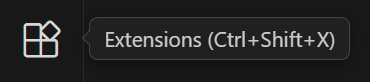
\includegraphics[scale=.75]{assets/vscode_extension.png}
\caption{To open the Extensions tab in VS Code, click the icon located on the toolbar on the left, or press \texttt{Ctrl+Shift+X}.}
\label{fig:vscode}
\end{figure}

\subsection{Open \kit{code.py} from the \kit{CIRCUITPY} drive}
In Visual Studio Code, select \textbf{File $\rightarrow$ Open Folder} and open the removable drive labeled \kit{CIRCUITPY}. Then open the file \kit{code.py}.

\begin{warningbox}
On the Bluefruit, only the file named \kit{code.py} runs automatically. Code placed in other files will not run unless it is explicitly imported by \kit{code.py}. To rerun the current program, simply save \kit{code.py} again with \textbf{Ctrl+S} or \textbf{File $\rightarrow$ Save}.
\end{warningbox}

To view printed output from your program, open the serial monitor in VS Code. One workable path is:
\begin{center}
\textbf{Terminal $\rightarrow$ New Terminal $\rightarrow$ SERIAL MONITOR $\rightarrow$ Start Monitoring}
\end{center}

\subsection{Short temperature-sensor example}
The onboard temperature sensor is available through the Circuit Playground helper library. Replace the contents of \kit{code.py} with the example in Figure~\ref{fig:temp}, save the file, and verify that the serial monitor reports temperature once every second.

Note that the sensor reports temperature in degrees Celsius, so we convert to degrees Fahrenheit in software.

\begin{figure}[H]
\centering
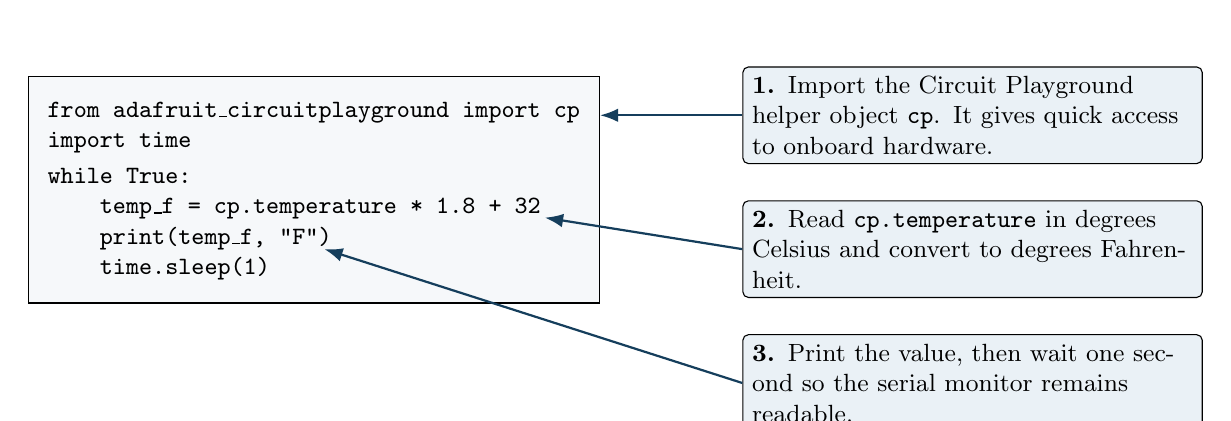
\begin{tikzpicture}[>=Latex, font=\small]
    \node[draw, fill=CodeBg, anchor=north west, inner sep=7pt, align=left] (code) at (0,0) {%
    \begin{tabular}{@{}l@{}}
    \texttt{from adafruit\_circuitplayground import cp}\\
    \texttt{import time}\\[0.2em]
    \texttt{while True:}\\
    \texttt{\ \ \ \ temp\_f = cp.temperature * 1.8 + 32}\\
    \texttt{\ \ \ \ print(temp\_f, "F")}\\
    \texttt{\ \ \ \ time.sleep(1)}
    \end{tabular}};

    \node[draw, fill=SoftAccent, rounded corners=2pt, text width=5.6cm, align=left] (c1) at (12,-0.5) {\textbf{1.} Import the Circuit Playground helper object \kit{cp}. It gives quick access to onboard hardware.};
    \node[draw, fill=SoftAccent, rounded corners=2pt, text width=5.6cm, align=left] (c2) at (12,-2.2) {\textbf{2.} Read \kit{cp.temperature} in degrees Celsius and convert to degrees Fahrenheit.};
    \node[draw, fill=SoftAccent, rounded corners=2pt, text width=5.6cm, align=left] (c3) at (12,-3.9) {\textbf{3.} Print the value, then wait one second so the serial monitor remains readable.};

    \draw[<-,Accent,thick] ($(code.north east)+(0,-0.5)$) -- (c1.west);
    \draw[<-,Accent,thick] ($(code.north east)+(-0.7,-1.8)$) -- (c2.west);
    \draw[<-,Accent,thick] ($(code.north east)+(-3.5,-2.2)$) -- (c3.west);
\end{tikzpicture}
\caption{Example printing ambient temperature at 1 Hz using the onboard thermometer.}\label{fig:temp}
\end{figure}

\begin{notebox}
Touch the board near the temperature sensor to make the reported temperature rise slightly. That is a simple sanity check that your code is reading a live sensor rather than stale output.
\end{notebox}

\subsection{Short NeoPixel example}
The ten onboard NeoPixels can be set to any RGB color using a three-number tuple \kit{(red, green, blue)}. Each value ranges from 0 to 255.

\begin{figure}[H]
\centering
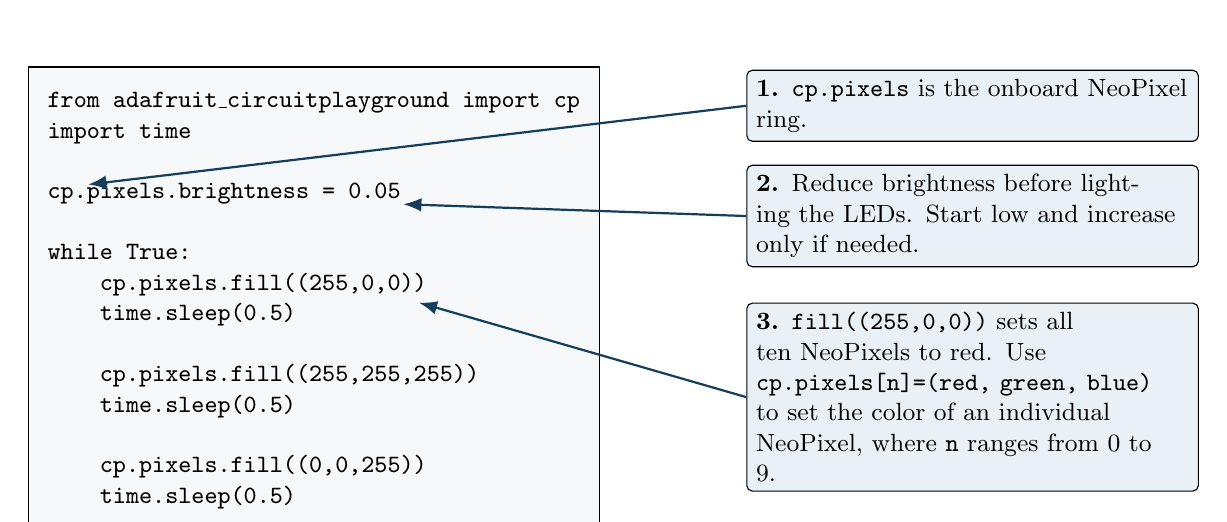
\begin{tikzpicture}[>=Latex, font=\small]
\node[draw, fill=CodeBg, anchor=north west, inner sep=7pt, align=left] (code) at (0,0) {%
\begin{tabular}{@{}l@{}}
\texttt{from adafruit\_circuitplayground import cp}\\
\texttt{import time}\\ \\
\texttt{cp.pixels.brightness = 0.05}\\ \\
\texttt{while True:}\\
\texttt{\ \ \ \ cp.pixels.fill((255,0,0))}\\
\texttt{\ \ \ \ time.sleep(0.5)}\\  \\
\texttt{\ \ \ \ cp.pixels.fill((255,255,255))}\\
\texttt{\ \ \ \ time.sleep(0.5)}\\ \\
\texttt{\ \ \ \ cp.pixels.fill((0,0,255))}\\
\texttt{\ \ \ \ time.sleep(0.5)}\\
\end{tabular}};
\node[draw, fill=SoftAccent, rounded corners=2pt, text width=5.5cm, align=left] (n1) at (12,-0.5) {\textbf{1.} \kit{cp.pixels} is the onboard NeoPixel ring.};
\node[draw, fill=SoftAccent, rounded corners=2pt, text width=5.5cm, align=left] (n2) at (12,-1.9) {\textbf{2.} Reduce brightness before lighting the LEDs. Start low and increase only if needed.};
\node[draw, fill=SoftAccent, rounded corners=2pt, text width=5.5cm, align=left] (n3) at (12,-4.2) {\textbf{3.} \kit{fill((255,0,0))} sets all ten NeoPixels to red. Use \kit{cp.pixels[n]=(red, green, blue)} to set the color of an individual NeoPixel, where \kit{n} ranges from 0 to 9.};
\draw[<-,Accent,thick] ($(code.north east)+(-6.5,-1.5)$) -- (n1.west);
\draw[<-,Accent,thick] ($(code.north east)+(-2.5,-1.75)$) -- (n2.west);
\draw[<-,Accent,thick] ($(code.north east)+(-2.3,-3)$) -- (n3.west);
\end{tikzpicture}
\caption{Minimal NeoPixel example.}
\end{figure}

\subsection{Use GenAI to combine temperature and NeoPixels}
Give a GenAI tool the temperature example and the NeoPixel example. Ask it to create a single CircuitPython program that changes the NeoPixel color with temperature according to the following map:
\begin{center}
\textbf{70 \si{\degree F} $\rightarrow$ Blue} \hspace{2em} \textbf{90 \si{\degree F} $\rightarrow$ Red}
\end{center}
You can use the prompt below as a starting point.

\begin{calloutbox}{Suggested GenAI prompt}
I am using CircuitPython on an Adafruit Circuit Playground Bluefruit. Combine these two code fragments into one working \kit{code.py}. The program should read the current temperature once per second, convert it to Fahrenheit, print the temperature to the serial monitor, and set all ten NeoPixels to a color between blue at 70 F and red at 90 F. Clamp any value below 70 F to blue and any value above 90 F to red. Use the \kit{adafruit\_circuitplayground} helper library.
\end{calloutbox}

\newpage
\section{Logging data to a microSD card}

\subsection{Connect the microSD breakout board}
Connect the microSD breakout board to the carrier PCB using jumper wires and the pin mappings specified in Table~\ref{table:microsd}. You may have to solder headers onto the microSD breakout board if no headers have already been soldered. See Figure~\ref{fig:microsd} for proper orientation and placement.

\begin{figure}[H]
\centering
\begin{subfigure}[t]{0.34\linewidth}
    \centering
    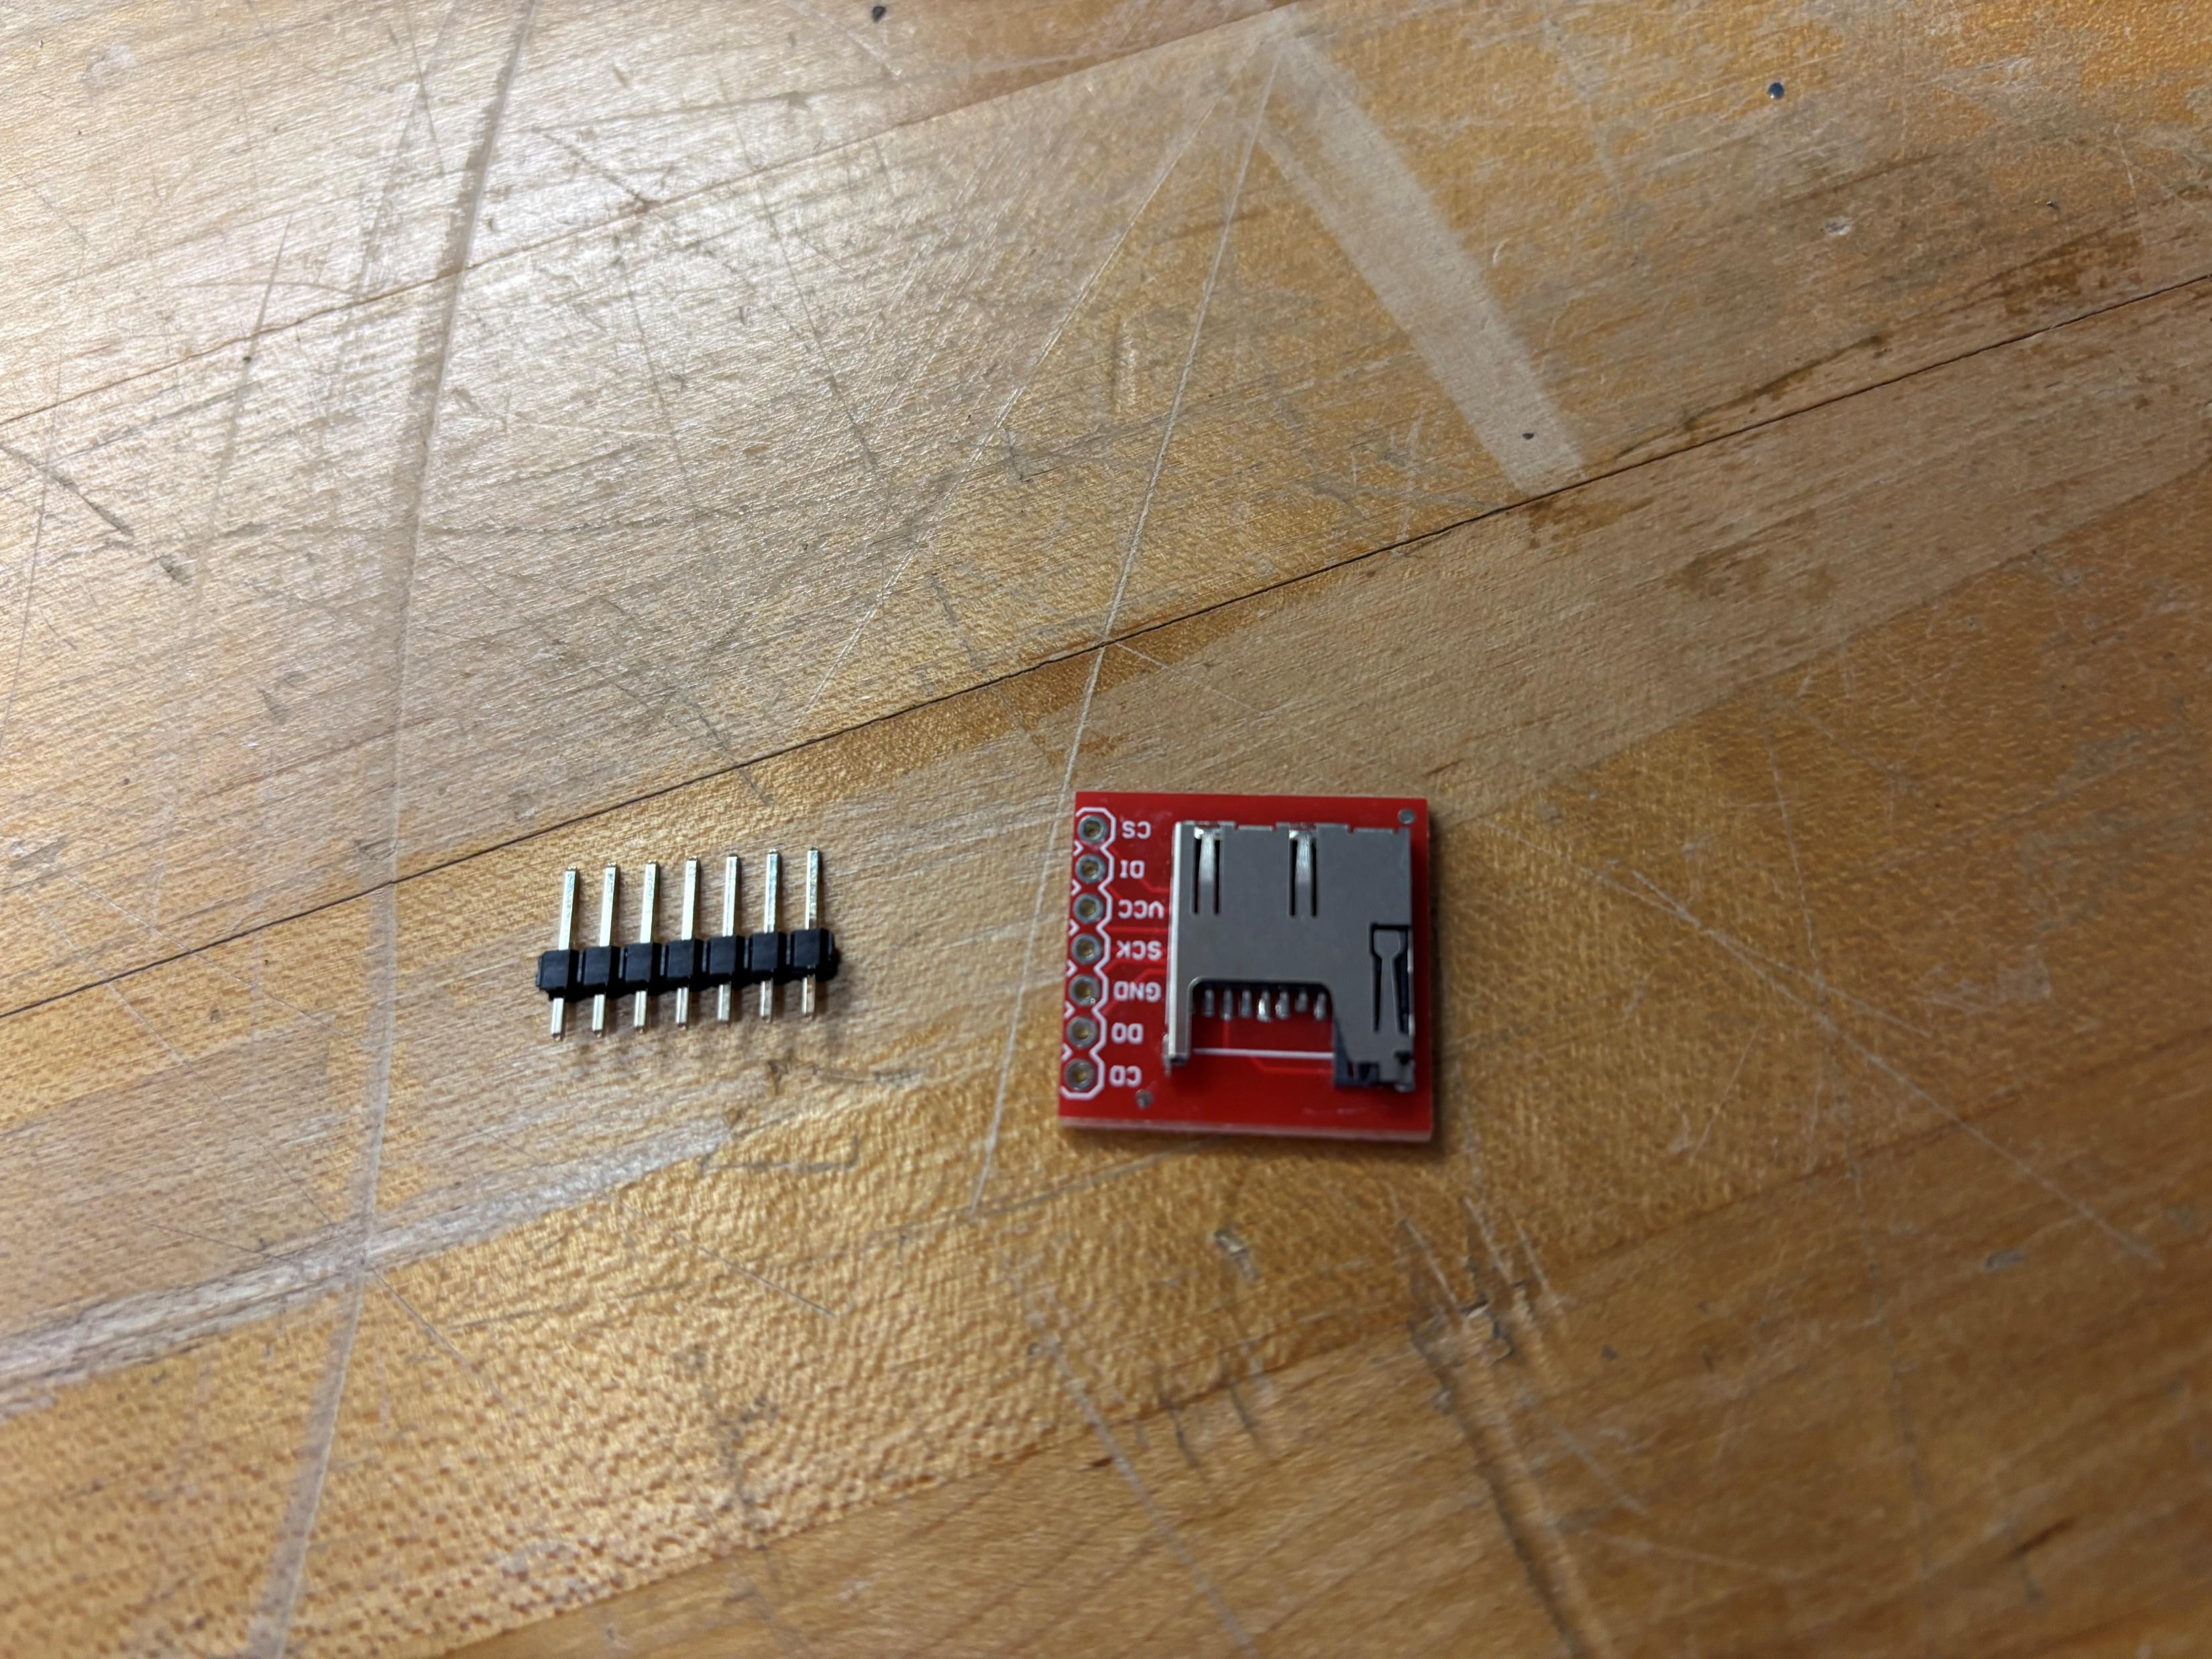
\includegraphics[width=\linewidth]{assets/sd_parts.jpg}
    \caption{microSD breakout and header before assembly.}
\end{subfigure}
\hfill
\begin{subfigure}[t]{0.23\linewidth}
    \centering
    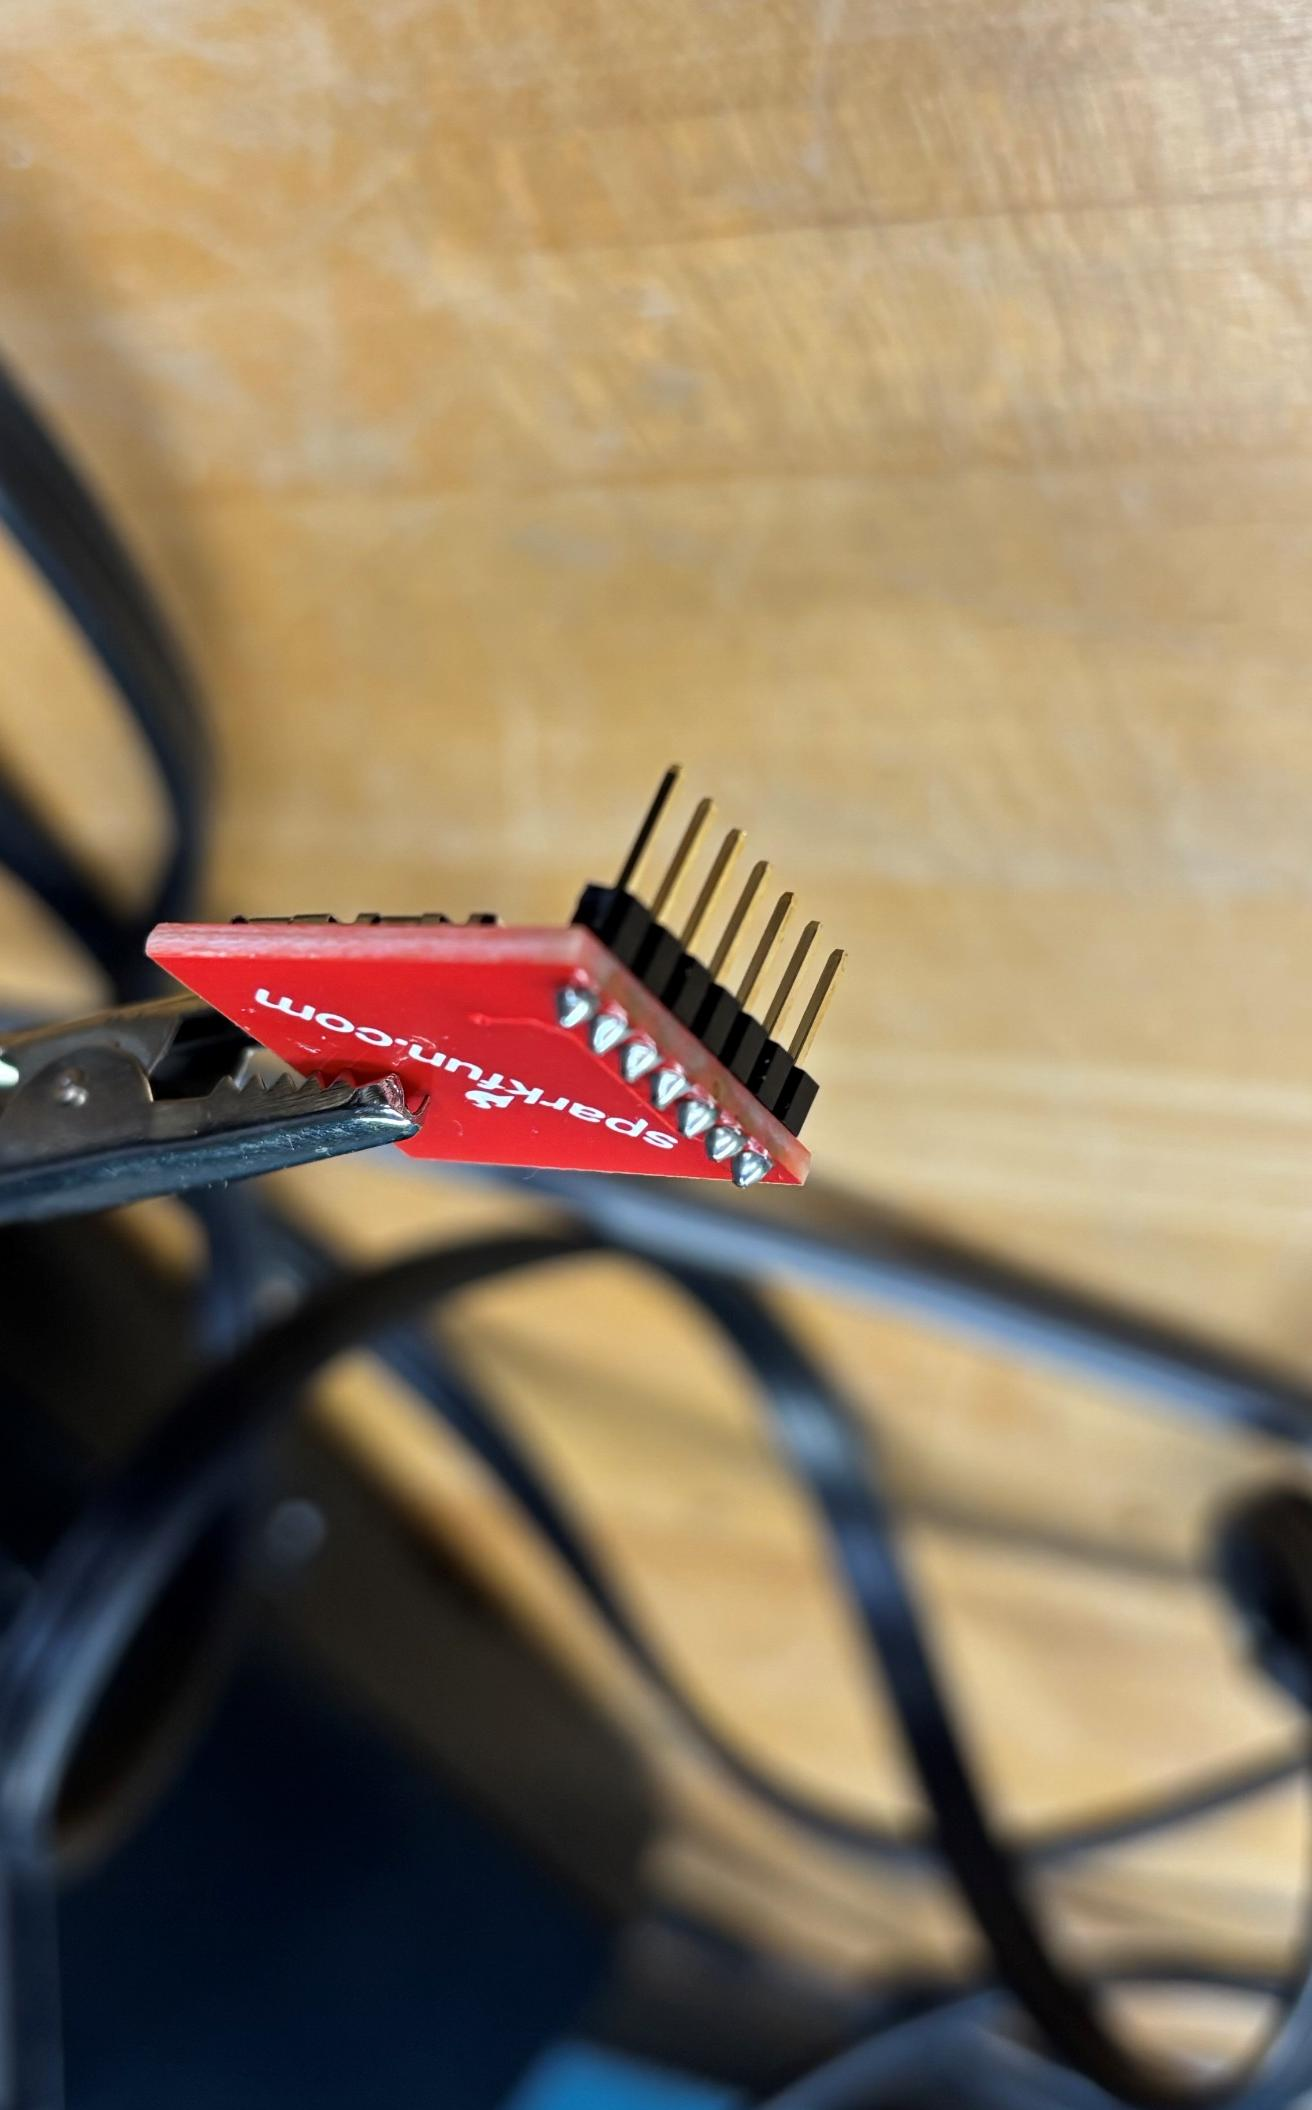
\includegraphics[width=\linewidth]{assets/sd_soldered_close.jpg}
    \caption{Header soldered onto the breakout.}
\end{subfigure}
\hfill
\begin{subfigure}[t]{0.23\linewidth}
    \centering
    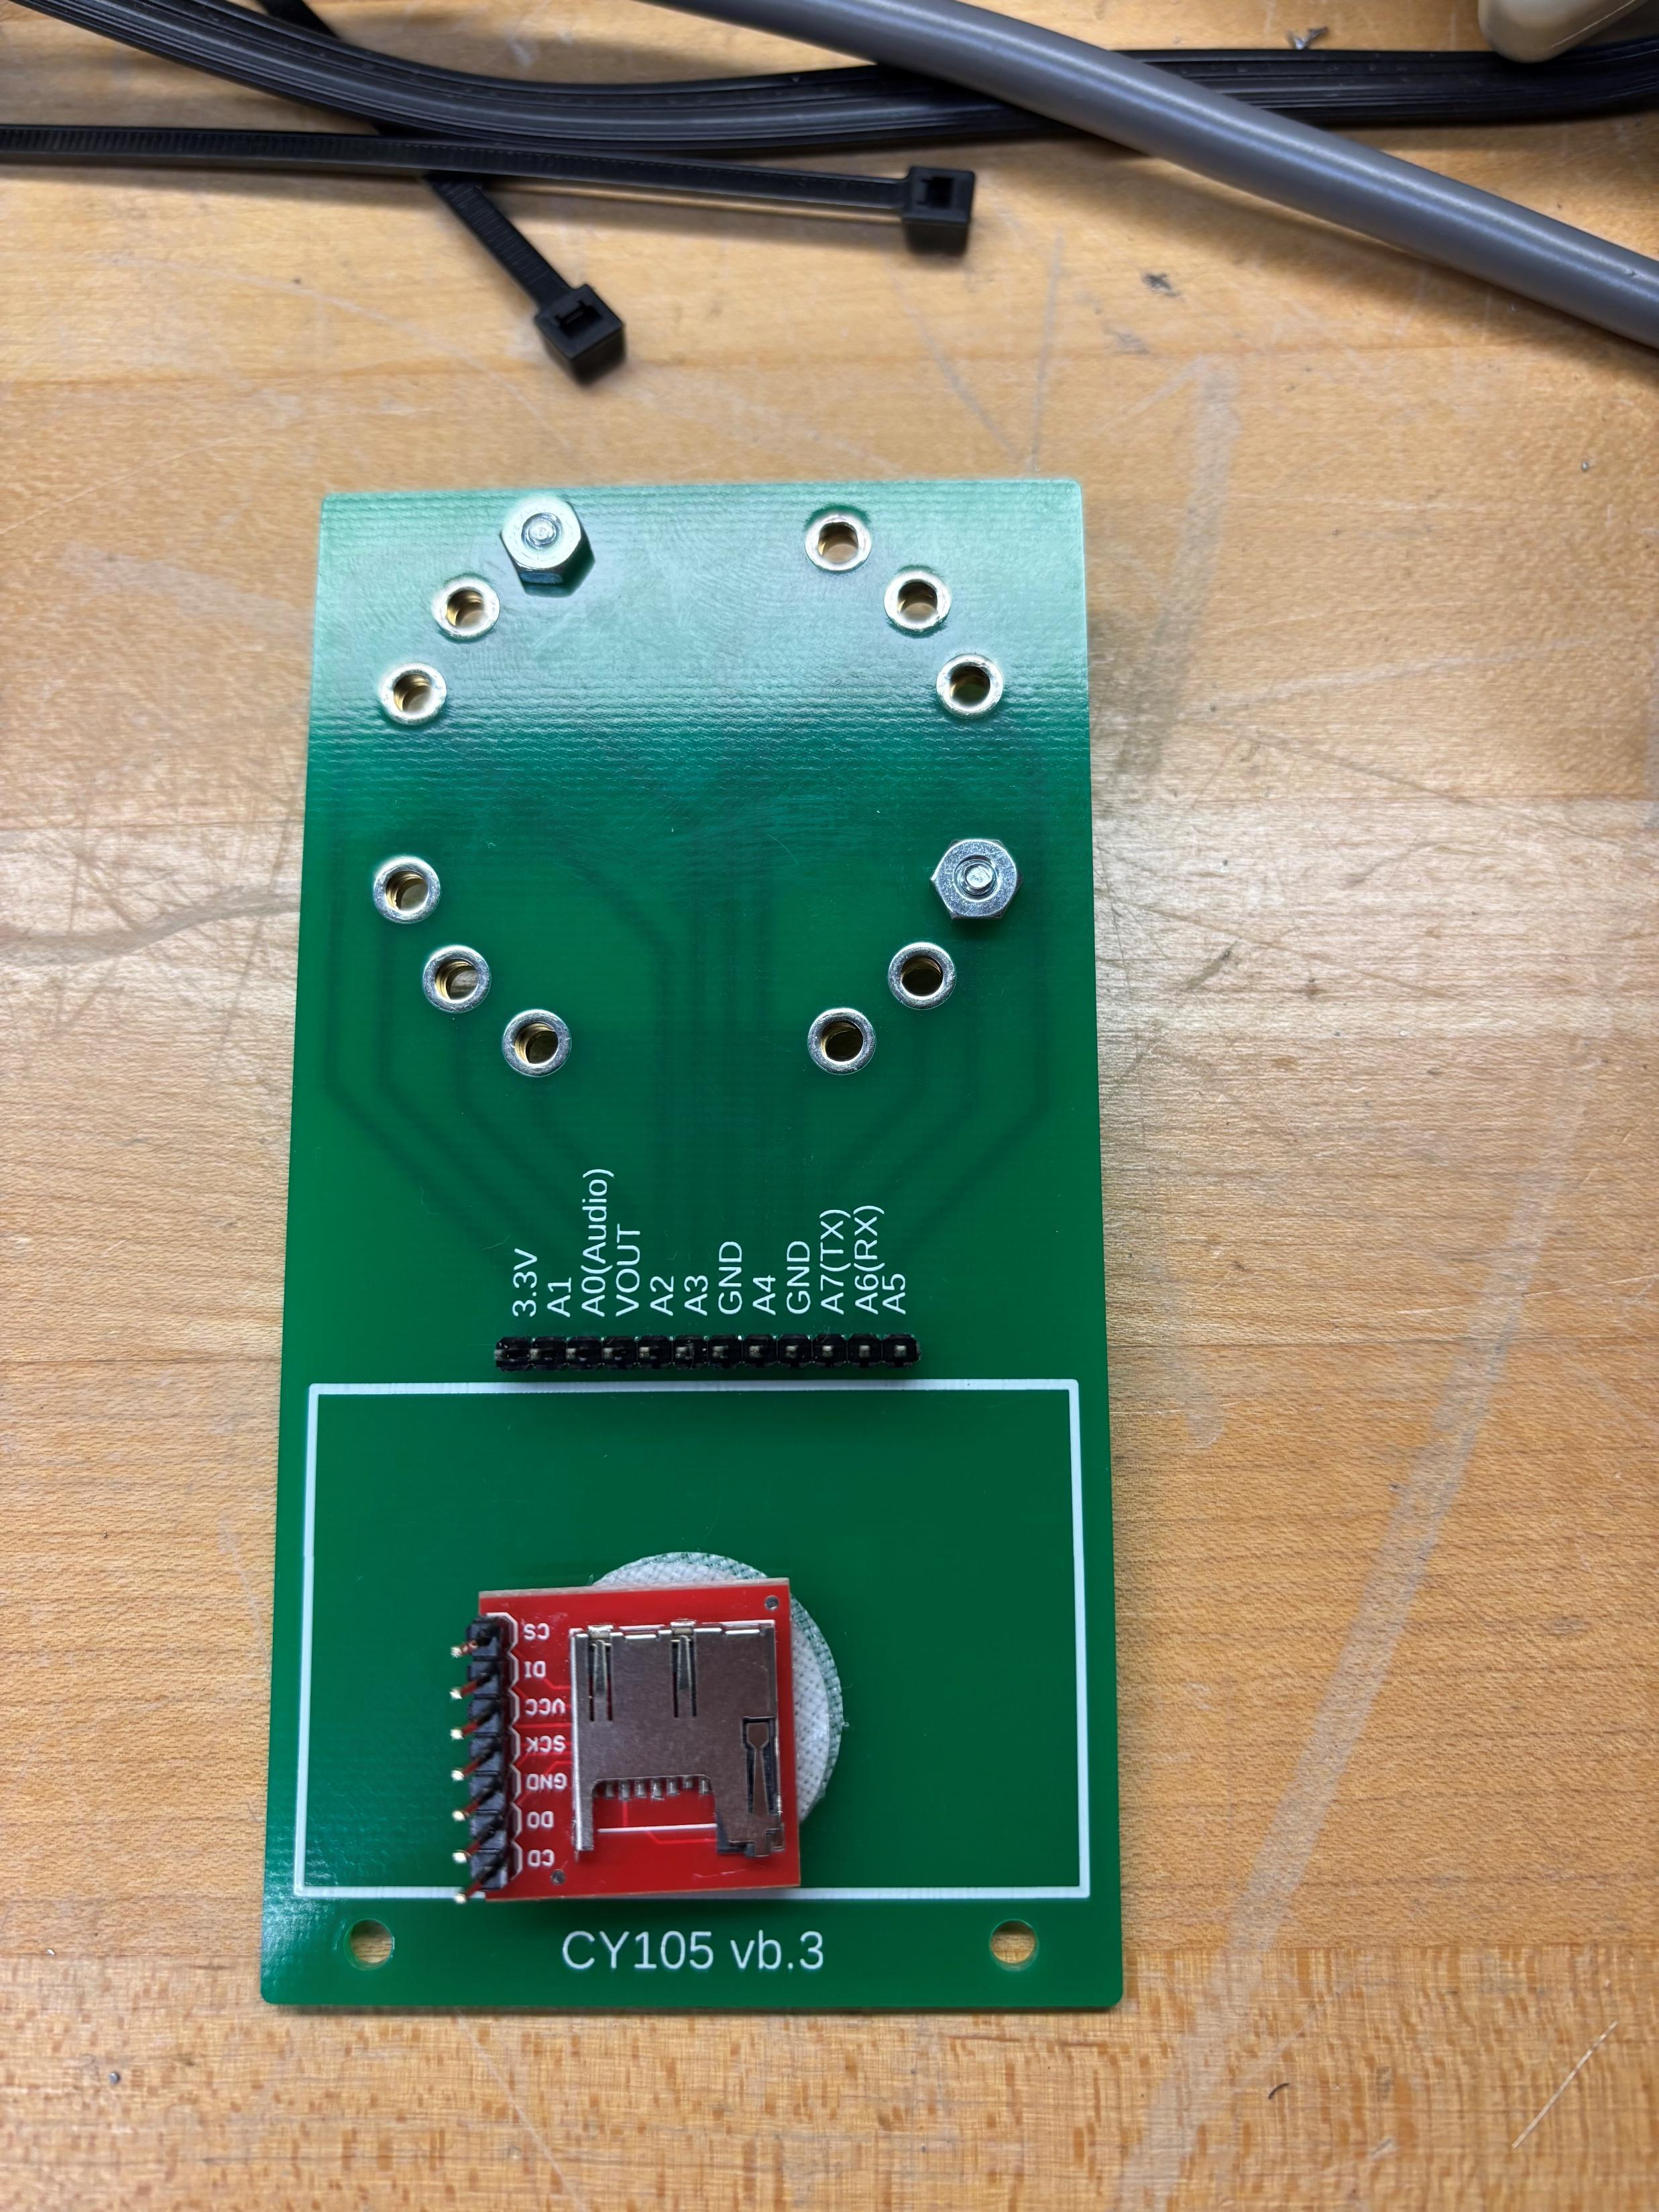
\includegraphics[width=\linewidth]{assets/sd_mounted.jpg}
    \caption{Breakout installed on the carrier PCB.}
\end{subfigure}
\caption{microSD breakout preparation. Do not solder the header with a card inserted.}\label{fig:microsd}
\end{figure}

\begin{table}[H]
\centering
\caption{Recommended microSD wiring for this lab}\label{table:microsd}
\renewcommand{\arraystretch}{1.25}
\begin{tabular}{>{\bfseries}p{1in} p{1.2in} p{1.5in} p{2.1in}}
\toprule
Signal & Bluefruit & microSD breakout & Function \\
\midrule
Ground & GND & GND & Common reference \\
3.3 V & 3.3V & VCC & Logic and card power \\
SPI clock & A3 & SCK & Serial clock \\
SPI MISO & A2 & DO & Data, card to microcontroller \\
SPI MOSI & A1 & DI & Data, microcontroller to card \\
Chip select & A0 (Audio / D12) & CS & Enable SPI communication \\
\bottomrule
\end{tabular}
\end{table}

\begin{notebox}
This wiring choice leaves the default I2C pins and UART pins open for the I2C and GPS loaner sensors. It does, however, use the \kit{AUDIO / D12} pin for chip select, so you should not plan to use the onboard speaker at the same time as the SD card with this exact wiring. The \kit{/sd} mount point needed by CircuitPython was already created by the diagnostics package during the reflash process.
\end{notebox}

\subsection{Write one line of text to a file}
Use the example below to mount the SD card and write a single line of text to a file. After the program runs, remove the microSD card and inspect it with a card reader.

\begin{lstlisting}
import board
import busio
import digitalio
import adafruit_sdcard
import storage

# Setup SPI for the SD card
spi = busio.SPI(clock=board.A3, MOSI=board.A1, MISO=board.A2)

# Setup CS (Chip Select) pin
cs = digitalio.DigitalInOut(board.AUDIO)  # Use pin D12 for CS
cs.direction = digitalio.Direction.OUTPUT
cs.value = True  # Set CS high

# Create the SD card object
sd_card = adafruit_sdcard.SDCard(spi, cs)

# Mount the SD card
vfs = storage.VfsFat(sd_card)
storage.mount(vfs, "/sd")

# Create a new file and write to it
with open("/sd/hello.txt", "w") as f:
    f.write("Hello world!\n")

while True:
    pass  # Keep the program running
\end{lstlisting}

\paragraph{Check.} Save the file, let it run, then remove the microSD card and verify with a card reader that \kit{hello.txt} was written successfully.

\subsection{Use GenAI to build a temperature logger}
Now provide GenAI with the temperature example and the SD-card example. Ask it to create a single \kit{code.py} that writes the current temperature to a text file once per second.

\begin{calloutbox}{Suggested GenAI prompt}
Combine these CircuitPython examples into one working \kit{code.py} for an Adafruit Circuit Playground Bluefruit. The program should mount the SD card, create or append to a text file, and write the current temperature in Fahrenheit once every second. Print the same line to the serial monitor. Keep the SD wiring exactly as shown in the starter code.
\end{calloutbox}

\section{Final project and equipment turn-in}

\subsection{Final project requirements}
Your final project must use \textbf{at least two sensor inputs}, \textbf{at least one output}, and generate at least 1000 data entries logged to the microSD card.

\subsubsection{Onboard Bluefruit sensors and I/O}
\begin{itemize}
    \item Temperature sensor
    \item Light sensor
    \item Accelerometer
    \item Microphone
    \item Buttons A \& B
    \item Slide switch
    \item Capacitive touch pads
    \item NeoPixels
    \item Speaker
    \item Red LED (D13)
\end{itemize}

\subsubsection{External sensors available for loan}
\begin{table}[H]
\small
\centering
\caption{Loaner sensors for final projects}
\renewcommand{\arraystretch}{1.2}
\begin{tabularx}{\linewidth}{p{3in} p{0.8in} X}
\toprule
Device & Interface & Notes \\
\midrule
Adafruit Ultimate GPS Breakout & UART & Best used outdoors or near a window; requires time to acquire a fix. \\
Adafruit VEML7700 Lux Sensor & I2C & Ambient light sensor. \\
Adafruit LSM303AGR Accelerometer \& Compass & I2C & Reports both acceleration and magnetic field. \\
Adafruit SHT30 Humidity \& Temperature Sensor & I2C & Adds humidity plus a second temperature source. \\
Ohmite FSR01 Force Sensing Resistor & Analog & Variable resistance / pressure sensing. \\
Parallax Passive IR Sensor & Digital & Motion detection. \\
Parallax 2-Axis Joystick & Analog & Two-axis user input. \\
Parallax PING))) Ultrasonic Distance Sensor & Digital pulse & Distance measurement by ultrasonic echo timing. \\
Parallax LaserPING Rangefinder & Digital pulse & Optical distance measurement. \\
\bottomrule
\end{tabularx}
\end{table}

Starter code for each onboard capability appears in Appendix~\ref{app:onboard}. Starter code for each external loaner sensor appears in Appendix~\ref{app:offboard}.

\subsection{Equipment turn-in}
All loaned equipment must be turned in before the TEE. Return the carrier board, Bluefruit, breakout boards, jumper wires, and any other issued loaner items in complete and serviceable condition.

\newpage
\appendix

\section{Reference: Onboard I/O Starter Code}\label{app:onboard}
The examples in this appendix provide a starting point for using onboard I/O devices.

\subsection{Temperature sensor}

\begin{lstlisting}
import time
from adafruit_circuitplayground import cp

while True:
    temp_f = cp.temperature * 1.8 + 32
    print(temp_f, "F")
    time.sleep(1)
\end{lstlisting}

\subsection{Light sensor}

\begin{lstlisting}
import time
from adafruit_circuitplayground import cp

while True:
    print("Light:", cp.light)
    time.sleep(1)
\end{lstlisting}

\subsection{Accelerometer}

\begin{lstlisting}
import time
from adafruit_circuitplayground import cp

while True:
    x, y, z = cp.acceleration
    print((x, y, z))
    time.sleep(1)
\end{lstlisting}
\newpage
\subsection{Sound Level Sensor}

\begin{lstlisting}
import time
from adafruit_circuitplayground.bluefruit import cpb

while True:
    print("Sound level:", cpb.sound_level)
    time.sleep(0.1)
\end{lstlisting}

\subsection{Buttons A \& B}

\begin{lstlisting}
import time
from adafruit_circuitplayground import cp

while True:
    print("Button A:", cp.button_a, "Button B:", cp.button_b)
    time.sleep(0.1)
\end{lstlisting}

\subsection{Slide switch}

\begin{lstlisting}
import time
from adafruit_circuitplayground import cp

while True:
    print("Slide switch:", cp.switch)
    time.sleep(0.1)
\end{lstlisting}

\subsection{Capacitive touch pads}

%\paragraph{Pin connections} No external wiring is required. To test touch input, simply touch one of the exposed pads on the Bluefruit or the corresponding carrier-board header pin. The touch-capable pads are \texttt{A1}, \texttt{A2}, \texttt{A3}, \texttt{A4}, \texttt{A5}, \texttt{A6(RX)}, and \texttt{A7(TX)}. Do not use \texttt{A0(Audio)} for capacitive touch.

\begin{lstlisting}
import time
from adafruit_circuitplayground import cp

while True:
    if cp.touch_A1:
        print("Touched A1")
    if cp.touch_A2:
        print("Touched A2")
    if cp.touch_A3:
        print("Touched A3")
    if cp.touch_A4:
        print("Touched A4")
    if cp.touch_A5:
        print("Touched A5")
    if cp.touch_A6:
        print("Touched A6")
    if cp.touch_A7:
        print("Touched A7")
    time.sleep(0.1)
\end{lstlisting}

\subsection{NeoPixels}

\begin{lstlisting}
from adafruit_circuitplayground import cp
import time

cp.pixels.brightness = 0.05

while True:
    cp.pixels.fill((255,0,0))
    time.sleep(0.5)
    
    cp.pixels.fill((255,255,255))
    time.sleep(0.5)
    
    cp.pixels.fill((0,0,255))
    time.sleep(0.5)
\end{lstlisting}

\subsection{Speaker}

\begin{lstlisting}
import time
from adafruit_circuitplayground import cp

while True:
    cp.play_tone(440, 0.25)
    time.sleep(0.25)
    cp.play_tone(660, 0.25)
    time.sleep(0.25)
\end{lstlisting}

\subsection{Red LED (D13)}

%\paragraph{Pin connections} No external wiring is required. This is the small red LED next to the USB connector, labeled \texttt{D13} on the Bluefruit.

\begin{lstlisting}
import time
from adafruit_circuitplayground import cp

while True:
    cp.red_led = True
    time.sleep(0.5)
    cp.red_led = False
    time.sleep(0.5)
\end{lstlisting}
\newpage
\section{Reference: External Sensor Starter Code}\label{app:offboard}
The examples in this appendix are for reference only. When required, copy the necessary library files provided in the reflash kit to the \kit{lib} folder on \kit{CIRCUITPY}. The pin connections show the mapping from the sensors to ($\rightarrow$) the Bluefruit. Note that you will have to reassign some of the pins in your project to deconflict them with the microSD breakout board.

\subsection{Adafruit Ultimate GPS Breakout}
\paragraph{Pin connections} \texttt{TX} $\rightarrow$ \texttt{A6 (RX)}, \texttt{RX} $\rightarrow$ \texttt{A7 (TX)}, \texttt{VIN} $\rightarrow$ \texttt{3.3V}, \texttt{GND} $\rightarrow$ \texttt{GND}.

\begin{lstlisting}
import time
import board
import busio
import adafruit_gps

uart = busio.UART(board.TX, board.RX, baudrate=9600, timeout=10)
gps = adafruit_gps.GPS(uart, debug=False)
gps.send_command(b"PMTK314,0,1,0,1,0,0,0,0,0,0,0,0,0,0,0,0,0,0,0")
gps.send_command(b"PMTK220,1000")

last_print = time.monotonic()
while True:
    gps.update()
    current = time.monotonic()
    if current - last_print >= 1.0:
        last_print = current
        if not gps.has_fix:
            print("Waiting for fix...", gps.satellites, "in view")
            continue
        print("=" * 40)
        print(
            "Fix timestamp: {}/{}/{} {:02}:{:02}:{:02}".format(
                gps.timestamp_utc.tm_mon,
                gps.timestamp_utc.tm_mday,
                gps.timestamp_utc.tm_year,
                gps.timestamp_utc.tm_hour,
                gps.timestamp_utc.tm_min,
                gps.timestamp_utc.tm_sec,
            )
        )
        print("Latitude: {0:.6f} degrees".format(gps.latitude))
        print("Longitude: {0:.6f} degrees".format(gps.longitude))
        print(
            "Precise Latitude: {} degs, {:2.4f} mins".format(
                gps.latitude_degrees, gps.latitude_minutes
            )
        )
        print(
            "Precise Longitude: {} degs, {:2.4f} mins".format(
                gps.longitude_degrees, gps.longitude_minutes
            )
        )
        print("Fix quality: {}".format(gps.fix_quality))
        if gps.satellites is not None:
            print("# satellites: {}".format(gps.satellites))
        if gps.altitude_m is not None:
            print("Altitude: {} meters".format(gps.altitude_m))
        if gps.speed_knots is not None:
            print("Speed: {} knots".format(gps.speed_knots))
        if gps.speed_kmh is not None:
            print("Speed: {} km/h".format(gps.speed_kmh))
        if gps.track_angle_deg is not None:
            print("Track angle: {} degrees".format(gps.track_angle_deg))
        if gps.horizontal_dilution is not None:
            print("Horizontal dilution: {}".format(gps.horizontal_dilution))
        if gps.height_geoid is not None:
            print("Height geoid: {} meters".format(gps.height_geoid))
\end{lstlisting}

\subsection{Adafruit VEML7700 Lux Sensor}
\paragraph{Pin connections} \texttt{VCC} $\rightarrow$ \texttt{3.3V}, \texttt{GND} $\rightarrow$ \texttt{GND}, \texttt{SCL} $\rightarrow$ \texttt{SCL/A4}, \texttt{SDA} $\rightarrow$ \texttt{SDA/A5}.

\begin{lstlisting}
import time
import board
import adafruit_veml7700

i2c = board.I2C()
veml7700 = adafruit_veml7700.VEML7700(i2c)

while True:
    print("Ambient light:", veml7700.light)
    time.sleep(0.1)
\end{lstlisting}

\subsection{Adafruit LSM303AGR Accelerometer and Compass}
\paragraph{Pin connections} \texttt{VIN} $\rightarrow$ \texttt{3.3V}, \texttt{GND} $\rightarrow$ \texttt{GND}, \texttt{SCL} $\rightarrow$ \texttt{A4}, \texttt{SDA} $\rightarrow$ \texttt{A5}.

\begin{lstlisting}
import time
import board
import adafruit_lsm303_accel
import adafruit_lis2mdl

i2c = board.I2C()
accelerometer = adafruit_lsm303_accel.LSM303_Accel(i2c)
magnetometer = adafruit_lis2mdl.LIS2MDL(i2c)

while True:
    acc_x, acc_y, acc_z = accelerometer.acceleration
    mag_x, mag_y, mag_z = magnetometer.magnetic

    print(
        "Acceleration (m/s^2): ({0:10.3f}, {1:10.3f}, {2:10.3f})".format(
            acc_x, acc_y, acc_z
        )
    )
    print(
        "Magnetometer: ({0:10.3f}, {1:10.3f}, {2:10.3f})".format(
            mag_x, mag_y, mag_z
        )
    )
    print("")
    time.sleep(1.0)
\end{lstlisting}

\subsection{Adafruit SHT30 Humidity and Temperature Sensor}
\paragraph{Pin connections} \texttt{VIN} (red) $\rightarrow$ \texttt{3.3V}, \texttt{GND} (black) $\rightarrow$ \texttt{GND}, \texttt{SCL} (yellow) $\rightarrow$ \texttt{A4}, \texttt{SDA} (white) $\rightarrow$ \texttt{A5}.

\begin{lstlisting}
import time
import board
import adafruit_sht31d

i2c = board.I2C()
sensor = adafruit_sht31d.SHT31D(i2c)

loopcount = 0
while True:
    print("\nTemperature: %0.1f C" % sensor.temperature)
    print("Humidity: %0.1f %%" % sensor.relative_humidity)
    time.sleep(2)
\end{lstlisting}

\subsection{Ohmite FSR01 Force Sensing Resistor}
\paragraph{Pin connections} Use the FSR in a voltage-divider circuit. Connect one FSR terminal to \texttt{3.3V}. Connect the other FSR terminal to \texttt{A3}. Also connect a fixed resistor (for example, \SI{10}{\kilo\ohm}) from \texttt{A3} to \texttt{GND}. The analog input reads the midpoint of the divider.

As more force is applied, the FSR resistance changes, which changes the voltage seen at \texttt{A3}.

\begin{lstlisting}
import time
import board
import analogio

sig = analogio.AnalogIn(board.A3)

while True:
    val = sig.value / (2**16 - 1)
    print((val,))
    time.sleep(0.5)
\end{lstlisting}

\subsection{Parallax Passive IR Sensor}
\paragraph{Pin connections} \texttt{VCC} $\rightarrow$ \texttt{3.3V}, \texttt{GND} $\rightarrow$ \texttt{GND}, \texttt{OUT} $\rightarrow$ \texttt{A1}.

\begin{lstlisting}
import time
import board
import digitalio

sig = digitalio.DigitalInOut(board.A1)
sig.switch_to_input()

while True:
    print("PIR Sensor activated:", sig.value)
    time.sleep(0.5)
\end{lstlisting}

\subsection{Parallax 2-Axis Joystick}
\paragraph{Pin connections} \texttt{L/R+} $\rightarrow$ \texttt{3.3V}, one \texttt{L/R} pin $\rightarrow$ \texttt{A2}, one \texttt{U/D} pin $\rightarrow$ \texttt{A1}, \texttt{GND} $\rightarrow$ \texttt{GND}, \texttt{U/D+} $\rightarrow$ \texttt{3.3V}.

\begin{lstlisting}
import time
import board
import analogio

lr_pin = analogio.AnalogIn(board.A2)
ud_pin = analogio.AnalogIn(board.A1)

while True:
    lr = (lr_pin.value / (2**16 - 1)) * 2 - 1
    ud = (ud_pin.value / (2**16 - 1)) * 2 - 1

    print((lr, ud))
    time.sleep(0.5)
\end{lstlisting}

\subsection{Parallax PING))) Ultrasonic Distance Sensor}
\paragraph{Pin connections} \texttt{VIN} $\rightarrow$ \texttt{VOUT}, \texttt{GND} $\rightarrow$ \texttt{GND}, \texttt{SIG} $\rightarrow$ \texttt{A1}.

\begin{lstlisting}
import time
import board
import digitalio

sig = digitalio.DigitalInOut(board.A1)
oat = 15
mach1 = 331.5 + oat * 0.606
print(mach1)

while True:
    sig.switch_to_output()
    sig.value = False
    time.sleep(200e-6)
    sig.value = True
    time.sleep(5e-6)
    sig.value = False

    sig.switch_to_input()
    while not sig.value:
        pass

    start = time.monotonic_ns()
    while sig.value:
        pass
    end = time.monotonic_ns()

    pulse_width_ms = (end - start) / 1e6
    distance_mm = pulse_width_ms * mach1 / 2

    print((pulse_width_ms, distance_mm))
    time.sleep(0.1)
\end{lstlisting}

\subsection{Parallax LaserPING Rangefinder}
\paragraph{Pin connections} \texttt{VIN} $\rightarrow$ \texttt{3.3V}, \texttt{GND} $\rightarrow$ \texttt{GND}, \texttt{SIG} $\rightarrow$ \texttt{A1}.

\begin{lstlisting}
import time
import board
import digitalio

sig = digitalio.DigitalInOut(board.A1)

while True:
    sig.switch_to_output()
    sig.value = False
    time.sleep(200e-6)
    sig.value = True
    time.sleep(5e-6)
    sig.value = False

    sig.switch_to_input()
    while not sig.value:
        pass

    start = time.monotonic_ns()
    while sig.value:
        pass
    end = time.monotonic_ns()

    pulse_width_ms = (end - start) / 1e6
    distance_mm = pulse_width_ms * 171.5

    print((pulse_width_ms, distance_mm))
    time.sleep(0.1)
\end{lstlisting}

\end{document}
